


\ifnum 0\ifxetex 1\fi\ifluatex 1\fi=0 % if pdftex
 
\else % if luatex or xetex
  \usepackage{unicode-math}
  \defaultfontfeatures{Scale=MatchLowercase}
  \defaultfontfeatures[\rmfamily]{Ligatures=TeX,Scale=1}
\fi

\makeatletter
\@ifundefined{KOMAClassName}{% if non-KOMA class
  \IfFileExists{parskip.sty}{%
    
  }{% else
    \setlength{\parindent}{0pt}
    \setlength{\parskip}{6pt plus 2pt minus 1pt}}
}{% if KOMA class
  \KOMAoptions{parskip=half}}
\makeatother


\hypersetup{
  pdftitle={Praktická časť diplomovej práce},
  hidelinks,
  pdfcreator={LaTeX via pandoc}}
\urlstyle{same} % disable monospaced font for URLs

\newcommand{\VerbBar}{|}
\newcommand{\VERB}{\Verb[commandchars=\\\{\}]}
\DefineVerbatimEnvironment{Highlighting}{Verbatim}{commandchars=\\\{\}}
% Add ',fontsize=\small' for more characters per line

\definecolor{shadecolor}{RGB}{248,248,248}
\newenvironment{Shaded}{\begin{snugshade}}{\end{snugshade}}
\newcommand{\AlertTok}[1]{\textcolor[rgb]{0.94,0.16,0.16}{#1}}
\newcommand{\AnnotationTok}[1]{\textcolor[rgb]{0.56,0.35,0.01}{\textbf{\textit{#1}}}}
\newcommand{\AttributeTok}[1]{\textcolor[rgb]{0.77,0.63,0.00}{#1}}
\newcommand{\BaseNTok}[1]{\textcolor[rgb]{0.00,0.00,0.81}{#1}}
\newcommand{\BuiltInTok}[1]{#1}
\newcommand{\CharTok}[1]{\textcolor[rgb]{0.31,0.60,0.02}{#1}}
\newcommand{\CommentTok}[1]{\textcolor[rgb]{0.56,0.35,0.01}{\textit{#1}}}
\newcommand{\CommentVarTok}[1]{\textcolor[rgb]{0.56,0.35,0.01}{\textbf{\textit{#1}}}}
\newcommand{\ConstantTok}[1]{\textcolor[rgb]{0.00,0.00,0.00}{#1}}
\newcommand{\ControlFlowTok}[1]{\textcolor[rgb]{0.13,0.29,0.53}{\textbf{#1}}}
\newcommand{\DataTypeTok}[1]{\textcolor[rgb]{0.13,0.29,0.53}{#1}}
\newcommand{\DecValTok}[1]{\textcolor[rgb]{0.00,0.00,0.81}{#1}}
\newcommand{\DocumentationTok}[1]{\textcolor[rgb]{0.56,0.35,0.01}{\textbf{\textit{#1}}}}
\newcommand{\ErrorTok}[1]{\textcolor[rgb]{0.64,0.00,0.00}{\textbf{#1}}}
\newcommand{\ExtensionTok}[1]{#1}
\newcommand{\FloatTok}[1]{\textcolor[rgb]{0.00,0.00,0.81}{#1}}
\newcommand{\FunctionTok}[1]{\textcolor[rgb]{0.00,0.00,0.00}{#1}}
\newcommand{\ImportTok}[1]{#1}
\newcommand{\InformationTok}[1]{\textcolor[rgb]{0.56,0.35,0.01}{\textbf{\textit{#1}}}}
\newcommand{\KeywordTok}[1]{\textcolor[rgb]{0.13,0.29,0.53}{\textbf{#1}}}
\newcommand{\NormalTok}[1]{#1}
\newcommand{\OperatorTok}[1]{\textcolor[rgb]{0.81,0.36,0.00}{\textbf{#1}}}
\newcommand{\OtherTok}[1]{\textcolor[rgb]{0.56,0.35,0.01}{#1}}
\newcommand{\PreprocessorTok}[1]{\textcolor[rgb]{0.56,0.35,0.01}{\textit{#1}}}
\newcommand{\RegionMarkerTok}[1]{#1}
\newcommand{\SpecialCharTok}[1]{\textcolor[rgb]{0.00,0.00,0.00}{#1}}
\newcommand{\SpecialStringTok}[1]{\textcolor[rgb]{0.31,0.60,0.02}{#1}}
\newcommand{\StringTok}[1]{\textcolor[rgb]{0.31,0.60,0.02}{#1}}
\newcommand{\VariableTok}[1]{\textcolor[rgb]{0.00,0.00,0.00}{#1}}
\newcommand{\VerbatimStringTok}[1]{\textcolor[rgb]{0.31,0.60,0.02}{#1}}
\newcommand{\WarningTok}[1]{\textcolor[rgb]{0.56,0.35,0.01}{\textbf{\textit{#1}}}}

\makeatletter
\patchcmd\longtable{\par}{\if@noskipsec\mbox{}\fi\par}{}{}
\makeatother
% Allow footnotes in longtable head/foot
\IfFileExists{footnotehyper.sty}
\makeatletter
\def\maxwidth{\ifdim\Gin@nat@width>\linewidth\linewidth\else\Gin@nat@width\fi}
\def\maxheight{\ifdim\Gin@nat@height>\textheight\textheight\else\Gin@nat@height\fi}
\makeatother
% Scale images if necessary, so that they will not overflow the page
% margins by default, and it is still possible to overwrite the defaults
% using explicit options in \includegraphics[width, height, ...]{}
\setkeys{Gin}{width=\maxwidth,height=\maxheight,keepaspectratio}
% Set default figure placement to htbp
\makeatletter
\def\fps@figure{htbp}
\makeatother
\setlength{\emergencystretch}{3em} % prevent overfull lines
\providecommand{\tightlist}{%
  \setlength{\itemsep}{0pt}\setlength{\parskip}{0pt}}
\setcounter{secnumdepth}{5}

\makeatletter
\def\maxwidth{\ifdim\Gin@nat@width>\linewidth\linewidth\else\Gin@nat@width\fi}
\def\maxheight{\ifdim\Gin@nat@height>\textheight\textheight\else\Gin@nat@height\fi}
\makeatother

\title{Praktická časť diplomovej práce}
\author{}
\date{\vspace{-2.5em}}



\maketitle

\hypertarget{sprievodca-ekfmetriou}{%
\section{Sprievodca ekfmetriou}\label{sprievodca-ekfmetriou}}

Sprievodca ekonometriou má za úlohu priblížiť Vám ekonometriu, a pomôcť
Vám jej porozumieť. Sprievodcu píšem ako študent, ktorý sa ekonometriu
začal učiť sám, a sám si prešiel zdĺhavým procesom bádania a
usmerňovania. Sprievodca je zostrojený ako-tak súbežne s osnovou a
zadaniami, ktoré obdržíte na hodine. Nebudeme sa konkrétne držať
vypracovania zadaní, ale skôr princípmi, z ktorých zadania ťažia. Mnoho
študentov tento predmet nezaujíma, a zadania vypracujú okopírovaním
postupov starších spolužiakov, nuž, pochopiť ekonometriu a jej postupy
nie je vôbec jednoduché, a dokážem pochopiť, keď si študenti hľadajú
skratky. Na druhú stranu, ekonometria predstavuje skvelú vstupnú bránu
do sveta analytiky. Človek je zavalený Machine Learningom, Data Sciencom
a AI-čkom, nuž až po sfúknutí pozlátka zistí, že je to zmes matematiky,
štatistiky a počítačovej vedy. Ekonometria je teda skvelou výhovorkou,
ako oprášiť matematiku, doučiť sa štatistiku, a naučiť sa troška
programovania. R-ko sa môže zdať ako jazyk, ktorý žije v tieni Pythonu,
avšak, akoby nejedna Dominika vedela dosvedčiť, netreba sa nechať
voviesť do omylu. R-ko je najvhodnejší programovací jazyk pre
štatistikov, Google ho zahrnul do najnovších kurzov Google Analytics.
Mojou úlohou je pomôcť Vám prekonať problém, ktorý som na začiatku
svojej cesty ekonometriou vôbec nepovažoval za problém, a to množstvo
materiálov, ktoré zavalí študenta. Pomôžem Vám postupne poskladať skladačku
konceptov a teórií, na ktorých ekonometria stojí. Náročnosť
prezentovania konceptov bude prispôsobená. Nehnevajte sa, keď neskôr
objavíte niečo, čo som spomenúť mohol, ale nespomenul. Nemá zmysel
vysvetľovať odvodzovanie každého estimátora. Cieľom je poskytnúť
všeobecný náhľad ekonometrie, a pomôcť Vám pochopiť, a príjemnejšie
zvládnuť predmet Ekonometria.

\newpage

\hypertarget{zuxe1klady-programovania-v-r}{%
\section{Základy programovania v R}\label{zuxe1klady-programovania-v-r}}

\begin{quote}
Sprievodca je interaktívny, teda začneme stiahnutím a inštaláciou
\href{https://cran.r-project.org/mirrors.html}{R} a
\href{https://cran.r-project.org/mirrors.html}{RStudia}. R má samo o
sebe programovacie prostredie, avšak dnešným štandardom je používanie
intregrovaného vývojového prostredia (IDE) v podobe RStudia.
\end{quote}

\hypertarget{aritmetickuxe9-operuxe1tory}{%
\subsection{Aritmetické operátory}\label{aritmetickuxe9-operuxe1tory}}

\emph{Poďme teda rovno na vec. Začneme základnými funkciami.} R môžeme
používať ako kalkulačku, teda za pomoci klasických aritmetických
operátorov môžeme sčítať, odčítať, násobiť, deliť či umocňovať:

\begin{Shaded}
\begin{Highlighting}[]
\DecValTok{5} \OperatorTok{+}\StringTok{ }\DecValTok{5}
\end{Highlighting}
\end{Shaded}

\begin{verbatim}
## [1] 10
\end{verbatim}

\begin{Shaded}
\begin{Highlighting}[]
\DecValTok{5} \OperatorTok{-}\StringTok{ }\DecValTok{5}
\end{Highlighting}
\end{Shaded}

\begin{verbatim}
## [1] 0
\end{verbatim}

\begin{Shaded}
\begin{Highlighting}[]
\DecValTok{5} \OperatorTok{*}\StringTok{ }\DecValTok{5}
\end{Highlighting}
\end{Shaded}

\begin{verbatim}
## [1] 25
\end{verbatim}

\begin{Shaded}
\begin{Highlighting}[]
\DecValTok{5} \OperatorTok{/}\StringTok{ }\DecValTok{5}
\end{Highlighting}
\end{Shaded}

\begin{verbatim}
## [1] 1
\end{verbatim}

\begin{Shaded}
\begin{Highlighting}[]
\DecValTok{5}\OperatorTok{^}\DecValTok{2}
\end{Highlighting}
\end{Shaded}

\begin{verbatim}
## [1] 25
\end{verbatim}

R-ko dokáže používať aj ďalšie aritmetické operátory:

\begin{Shaded}
\begin{Highlighting}[]
\CommentTok{# zobrazí zvyšok z delenia}
\DecValTok{5} \OperatorTok\StringTok{ }\DecValTok{2}
\end{Highlighting}
\end{Shaded}

\begin{verbatim}
## [1] 1
\end{verbatim}

My sa budeme zapodievať len tým, s čím sa na cvičeniach stretneme. Našou
úlohou nie je naučiť sa dokonalo ovládať R, ale naučiť sa používať ho v
dostatočnej miere, aby sme s ním zvládli to, čo budeme v najbližšej dobe
potrebovať.

\hypertarget{baluxedky}{%
\subsection{Balíky}\label{baluxedky}}

Okrem základných operátorov budeme využívať aj funkcie:

\begin{Shaded}
\begin{Highlighting}[]
\KeywordTok{mean}\NormalTok{(}\DecValTok{2}\NormalTok{, }\DecValTok{4}\NormalTok{, }\DecValTok{6}\NormalTok{)}
\end{Highlighting}
\end{Shaded}

\begin{verbatim}
## [1] 2
\end{verbatim}

\begin{Shaded}
\begin{Highlighting}[]
\KeywordTok{abs}\NormalTok{(}\OperatorTok{-}\DecValTok{5}\NormalTok{)}
\end{Highlighting}
\end{Shaded}

\begin{verbatim}
## [1] 5
\end{verbatim}

\begin{Shaded}
\begin{Highlighting}[]
\KeywordTok{sqrt}\NormalTok{(}\DecValTok{8}\NormalTok{)}
\end{Highlighting}
\end{Shaded}

\begin{verbatim}
## [1] 2.828427
\end{verbatim}

Tieto funkcie sa nachádzajú v balíkoch, ktoré si môžeme predstaviť ako
také Addony. R figuruje balíkmi, ktoré sú predinštalované, a zahŕňajú
najpoužívanejšie a najzákladnejšie funkcie. Vyššie použíté funkcie sa
nachádzajú v balíku base. To, v akom balíku sa funkcia nachádza, zistíte
po napísaní funkcie:

~

\begin{figure}
\begin{center}

\includegraphics{diplomka obrazky/1.png},
\caption{Snímka obrazovky - funkcia mean.}
\source{Zdroj: Vlastná tvorba.}
\end{center}
\end{figure}
~

to však len za predpokladu, že už máte balík nainštalovaný. Ak narazíte
na názov funkcie, ktorú chcete použiť, avšak nemáte nainštalovaný balík
a chcete zistiť jeho názov, buď si funkciu zadajte do Google, alebo
napíšte do konzoly:

\begin{Shaded}
\begin{Highlighting}[]
\CommentTok{# ??meno funkcie}
\NormalTok{??mean}
\end{Highlighting}
\end{Shaded}

My budeme často využívať predinštalované balíky \textbf{base} a
\textbf{stats}, avšak za pochodu si budeme inštalovať aj ďalšie balíky,
s ktorými sa na cvičeniach stretnete. Nový balík je potrebné prv
nainštalovať a potom ho načítať do prostredia.

\begin{Shaded}
\begin{Highlighting}[]
\CommentTok{# Stiahneme a nainštalujeme pomocou R konzoly a funkcie}
\CommentTok{# install.packages()}
\CommentTok{# ! Názov balíka je citlivý na veľkosť písma.}
\CommentTok{# ! Názov musí byť v úvodzovkách.}

\KeywordTok{install.packages}\NormalTok{(}\StringTok{"fBasics"}\NormalTok{)}

\CommentTok{# Po nainštalovaní máme balík stiahnutý v našom PC, a tento príkaz už}
\CommentTok{# viac nepoužívame. Ak však chceme funkcie z balíka použiť, musíme po}
\CommentTok{# zapnutí R-ka balík načítať príkazom.}

\KeywordTok{library}\NormalTok{(fBasics)}

\CommentTok{# ! tu už úvodzovky nie sú potrebné}
\end{Highlighting}
\end{Shaded}

\begin{quote}
\emph{Pri inštalovaní názov balíka zabalíme do úvodzoviek. Pri jeho
načítaní pomocou library() už úvodzovky nepíšeme. Na pohovor si vezmeme
oblek (úvodzovky), ale po prijatí už chodíme do práce bez obleku.}
\end{quote}

\hypertarget{objekty}{%
\subsection{Objekty}\label{objekty}}

Často chceme vyrátané výsledky znova použiť, a preto by bolo vhodné si
ich niekde uložiť. Na ukladanie a uskladnenie výsledkov slúžia objekty.
Každý objekt má meno a obsah. Meno si môžeme zadať akékoľvek, musí však:

\begin{itemize}
\tightlist
\item
  začínať malým alebo veľkým písmenom a nie číslom
\item
  obsahovať iba čísla, písmená alebo niektoré špeciálne znaky ako
  \("."\) či "\_".
\end{itemize}

\begin{quote}
\emph{Nezabúdajme, že R je case sensitive (rozlišuje veľké a malé
písmená).}
\end{quote}

Povedzme že chceme vytvoriť objekt \textbf{a} a priradiť mu hodnotu
\(2 + 2\). Na priradenie obsahu je možné použiť \("="\), avšak
štandardom je používanie \("<-"\).

\begin{quote}
\emph{Znak \textless- nie je nutné písať dvoma znakmi, používa sa na to
skratka \textbf{``ľavý Alt'' a ``-''}. Na SK klávesnici nájdeme znak
naľavo od pravého Shiftu, na EN klávesnici zvyčajne naľavo od Backspacu.
Osobne programujem s EN klávesnicou, nech som použíteľný v akomkoľvek
štáte bez potreby inštalovať SK klávesnicu.}
\end{quote}

\begin{Shaded}
\begin{Highlighting}[]
\CommentTok{# Priradíme teda objektu "a" výsledok "2 + 2".}
\NormalTok{a <-}\StringTok{ }\DecValTok{2} \OperatorTok{+}\StringTok{ }\DecValTok{2}

\CommentTok{# Po napísaní názvu objektu do konzoly, konzola ukáže už len výsledok.}
\NormalTok{a}
\end{Highlighting}
\end{Shaded}

\begin{verbatim}
## [1] 4
\end{verbatim}

\begin{Shaded}
\begin{Highlighting}[]
\CommentTok{# Nové priradenie hodnoty starému objektu prepíše starú hodnotu.}
\NormalTok{a <-}\StringTok{ }\DecValTok{5} \OperatorTok{+}\StringTok{ }\DecValTok{5}

\NormalTok{a}
\end{Highlighting}
\end{Shaded}

\begin{verbatim}
## [1] 10
\end{verbatim}

S daným objektom môžeme pracovať, akoby to bola číselná hodnota.

\begin{Shaded}
\begin{Highlighting}[]
\NormalTok{a}\OperatorTok{^}\DecValTok{2}
\end{Highlighting}
\end{Shaded}

\begin{verbatim}
## [1] 100
\end{verbatim}

\hypertarget{vektory}{%
\subsection{Vektory}\label{vektory}}

Pre priradenie viacerých hodnôt vytvoríme vektor. Vektor vytvoríme
pomocou funkcie c() ako combine.

\begin{Shaded}
\begin{Highlighting}[]
\CommentTok{# Objektu "a" priradíme súbor čísel a vytvoríme z neho vektor.}
\NormalTok{a <-}\StringTok{ }\KeywordTok{c}\NormalTok{(}\DecValTok{5}\NormalTok{, }\DecValTok{1}\NormalTok{, }\DecValTok{4}\NormalTok{, }\DecValTok{2}\NormalTok{, }\DecValTok{3}\NormalTok{)}

\NormalTok{a}
\end{Highlighting}
\end{Shaded}

\begin{verbatim}
## [1] 5 1 4 2 3
\end{verbatim}

S vektormi dokážeme rôzne pracovať. Sčítavať, násobiť, aplikovať na ne
funkcie, všetko, čo nás napadne. Ups, čo nám napadne!

\begin{Shaded}
\begin{Highlighting}[]
\NormalTok{b <-}\StringTok{ }\KeywordTok{c}\NormalTok{(}\DecValTok{5}\NormalTok{, }\DecValTok{9}\NormalTok{, }\DecValTok{6}\NormalTok{, }\DecValTok{8}\NormalTok{, }\DecValTok{7}\NormalTok{)}
\NormalTok{a }\OperatorTok{+}\StringTok{ }\NormalTok{b}
\end{Highlighting}
\end{Shaded}

\begin{verbatim}
## [1] 10 10 10 10 10
\end{verbatim}

\begin{Shaded}
\begin{Highlighting}[]
\KeywordTok{min}\NormalTok{(a)}
\end{Highlighting}
\end{Shaded}

\begin{verbatim}
## [1] 1
\end{verbatim}

\begin{Shaded}
\begin{Highlighting}[]
\KeywordTok{sort}\NormalTok{(a)}
\end{Highlighting}
\end{Shaded}

\begin{verbatim}
## [1] 1 2 3 4 5
\end{verbatim}

\begin{Shaded}
\begin{Highlighting}[]
\KeywordTok{sum}\NormalTok{(a)}
\end{Highlighting}
\end{Shaded}

\begin{verbatim}
## [1] 15
\end{verbatim}

Je vhodné poznať pár špeciálnych funkcií na tvorbu vektorov. A to:

\begin{Shaded}
\begin{Highlighting}[]
\CommentTok{# sample(), seq() a rep()}
\end{Highlighting}
\end{Shaded}

Často si totižto potrebujete vytvoriť vektor hodnôt podľa vlastnej
potreby. Hm, to som veľmi nič nové nepovedal. Ale\ldots{} Čo vlastne
tieto funkcie robia? A ako to zistíme? Ak pracujete s úplne novou
funkciou, a máte už nainštalovaný balík, a taktiež ste ho už načítali do
knižnice cez \(library()\), je vhodné použiť \(?názovfunkcie\) alebo
\(help(názovfunkcie)\). Poskytne Vám to stručný popis, čo funkcia robí,
všetky jej argumeny a aj pár príkladov. Ak už ste však s funkciou
pracovali, ale nepamätáte si argumenty, rozpíšte funkciu, kliknite sa do
zátvoriek funkcie \(mean(tu.sa.kliknete)\), a stlačíte \(TAB\). Vyhodí
Vám to argumenty funkcie. Skúsime si to na funkcii \(sample()\).

~

\hypertarget{sample}{%
\subsubsection{sample()}\label{sample}}

\begin{figure}
\begin{center}
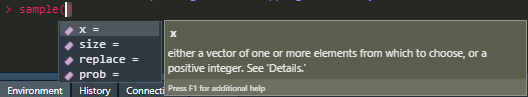
\includegraphics[width=0.85\textwidth,height=\textheight]{diplomka obrazky/2.png}
\caption{Snímka obrazovky - zobrazenie argumentov.}
\source{Zdroj: Vlastná tvorba.}

\end{center}
\end{figure}
~

Pri jednej z vecí, ktorú Vám chcem ukázať, budeme potrebovať vektor
výšky ľudí. Tak si ho teda vytvorme už teraz. Ešte predtým môžeme skúsiť
napísať do konzoly \(?sample\), čím zistíme, že funkcia \(sample()\) nám
náhodne vyberie hodnoty zo zadaného vektora.

~

\begin{figure}
\begin{center}

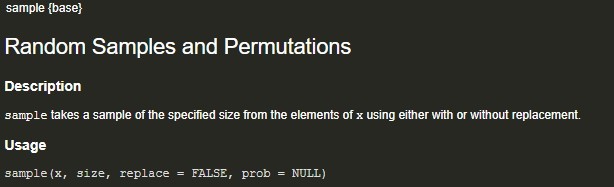
\includegraphics[width=0.8\textwidth,height=\textheight]{diplomka obrazky/3.png}
\caption{Snímka obrazovky - popis funkcie.}
\source{Zdroj: Vlastná tvorba.}

\end{center}
\end{figure}

~

\begin{Shaded}
\begin{Highlighting}[]
\CommentTok{# Ako prvé potrebujeme zadať "x", teda vektor hodnôt, z ktorých chceme} 
\CommentTok{# vyberať. Pre nás to budú hodnoty od 160 po 190, ktoré navolíme}
\CommentTok{# ako 160:190.}

\CommentTok{# 160:190 jednoducho vypíše hodnoty zaradom od 160 do 190, a}
\CommentTok{# sample() z nich náhodne vyberie nami určený počet hodnôt.}

\CommentTok{# "size" je počet hodnôt, aký ma funkcia vybrať.}
\CommentTok{# "replace", či môže vybrať jednu hodnotu viackrát, alebo ju má vylúčiť.}
\CommentTok{# "prob" použijeme, ak chceme priradiť istým hodnotám inú váhu.}

\NormalTok{vyska <-}\StringTok{ }\KeywordTok{sample}\NormalTok{(}\DataTypeTok{x =} \DecValTok{160}\OperatorTok{:}\DecValTok{190}\NormalTok{, }\DataTypeTok{size =} \DecValTok{10}\NormalTok{, }\DataTypeTok{replace =} \OtherTok{TRUE}\NormalTok{)}

\KeywordTok{print}\NormalTok{(vyska)}
\end{Highlighting}
\end{Shaded}

\begin{verbatim}
##  [1] 174 184 161 166 164 174 172 188 170 173
\end{verbatim}

\begin{quote}
\emph{Funkcia by fungovala, aj keby sme to napísali ako}
``sample(160:190, 10, TRUE)''. \emph{Je však vhodné písať aj argumenty.
Hlavne pri funkciách, ktoré nie sú veľmi bežné. Ak po Vás niekto bude
čítať kód, číta sa to lepšie.}
\end{quote}

\hypertarget{seq}{%
\subsubsection{seq()}\label{seq}}

Funkcia \(seq()\) vygeneruje sekvenciu čísel. Ako argumenty zadávame buď
\(od\), \(do\) a \(by\). Teda po akých inkrementoch bude daná sekvencia
narastať.

\begin{Shaded}
\begin{Highlighting}[]
\KeywordTok{seq}\NormalTok{(}\DataTypeTok{from =} \DecValTok{2}\NormalTok{, }\DataTypeTok{to =} \DecValTok{12}\NormalTok{, }\DataTypeTok{by =} \FloatTok{0.5}\NormalTok{)}
\end{Highlighting}
\end{Shaded}

\begin{verbatim}
##  [1]  2.0  2.5  3.0  3.5  4.0  4.5  5.0  5.5  6.0  6.5  7.0  7.5  8.0
## [14]  8.5  9.0 9.5 10.0 10.5 11.0 11.5 12.0
\end{verbatim}

~

\begin{quote}
\emph{V Rku používame na oddeľovanie desatiných miest bodku. Čiarkou
oddeľujeme argumenty. Taktiež nezabúdajte používať medzery. Jedná sa o
gramatiku programovania. Predsalen náš vyššie napísaný výraz vyzerá
lepšie ako} seq(from=2,to=12,by=0.5).
\end{quote}

~

\begin{Shaded}
\begin{Highlighting}[]
\CommentTok{# Zadáme "od", "do" a koľko časí má vektor mať.}
\KeywordTok{seq}\NormalTok{(}\DataTypeTok{from =} \DecValTok{4}\NormalTok{, }\DataTypeTok{to =} \DecValTok{10}\NormalTok{, }\DataTypeTok{length =} \DecValTok{4}\NormalTok{) }
\end{Highlighting}
\end{Shaded}

\begin{verbatim}
## [1]  4  6  8 10
\end{verbatim}

\begin{Shaded}
\begin{Highlighting}[]
\KeywordTok{seq}\NormalTok{(}\DataTypeTok{from =} \DecValTok{4}\NormalTok{, }\DataTypeTok{to =} \DecValTok{10}\NormalTok{, }\DataTypeTok{length =} \DecValTok{8}\NormalTok{)}
\end{Highlighting}
\end{Shaded}

\begin{verbatim}
## [1] 4.000000  4.857143  5.714286  6.571429  7.428571  8.285714
## [7] 9.142857 10.000000
\end{verbatim}

\newline

\begin{Shaded}
\begin{Highlighting}[]
\CommentTok{# Alternatívou je zadať "od", "po", a rozdeliť to po požadovaných}
\CommentTok{# kúskoch, na požadovanú dĺžku.}
\KeywordTok{seq}\NormalTok{(}\DataTypeTok{from =} \DecValTok{4}\NormalTok{, }\DataTypeTok{by =} \FloatTok{0.5}\NormalTok{, }\DataTypeTok{length =} \DecValTok{25}\NormalTok{)}
\end{Highlighting}
\end{Shaded}

\begin{verbatim}
##  [1] 4.0  4.5  5.0  5.5  6.0  6.5  7.0  7.5  8.0  8.5  9.0  9.5 10.0 
## [14] 10.5 11.0 11.5 12.0 12.5 13.0 13.5 14.0 14.5 15.0 15.5 16.0
\end{verbatim}

\hypertarget{rep}{%
\subsubsection{rep()}\label{rep}}

Funkcie \(rep()\) jednoducho zopakuje zadané číslo, alebo vektor,
x-krát.

\begin{Shaded}
\begin{Highlighting}[]
\KeywordTok{rep}\NormalTok{(}\DataTypeTok{x =} \DecValTok{1}\NormalTok{, }\DataTypeTok{times =} \DecValTok{10}\NormalTok{)}
\end{Highlighting}
\end{Shaded}

\begin{verbatim}
##  [1] 1 1 1 1 1 1 1 1 1 1
\end{verbatim}

\begin{Shaded}
\begin{Highlighting}[]
\KeywordTok{rep}\NormalTok{(}\DataTypeTok{x =} \KeywordTok{c}\NormalTok{(}\DecValTok{1}\NormalTok{, }\DecValTok{2}\NormalTok{, }\DecValTok{3}\NormalTok{), }\DataTypeTok{times =} \DecValTok{3}\NormalTok{)}
\end{Highlighting}
\end{Shaded}

\begin{verbatim}
## [1] 1 2 3 1 2 3 1 2 3
\end{verbatim}

\hypertarget{indexovanie}{%
\subsection{Indexovanie}\label{indexovanie}}

Indexovanie je v R-ku veľmi užitočný spôsob selektovania dát. Ide
jednoducho o výber súboru dát, zo súboru dát. Indexujeme za použitia
hranatých zátvoriek, ktoré bez medzery nalepíme k objektu, z ktorého
chceme dáta vybrať. Najjednoduchšie sa to vysvetľuje ukážkou. A
nezabúdajte, že R-ko začína od jednotky, nie od nuly. Aj keď nám,
ekonómom neprogramátorom to asi ani nepríde divné.

\begin{Shaded}
\begin{Highlighting}[]
\CommentTok{# Vytvorme si obyčajný číselný vektor.}
\NormalTok{obycajny_vektor <-}\StringTok{ }\KeywordTok{c}\NormalTok{(}\DecValTok{1}\OperatorTok{:}\DecValTok{10}\NormalTok{)}

\NormalTok{obycajny_vektor}
\end{Highlighting}
\end{Shaded}

\begin{verbatim}
##  [1]  1  2  3  4  5  6  7  8  9 10
\end{verbatim}

\begin{Shaded}
\begin{Highlighting}[]
\CommentTok{# Za použitia indexovania môžeme vybrať akúkoľvek hodnotu.}
\CommentTok{# My chceme vybrať prvú.}
\NormalTok{obycajny_vektor[}\DecValTok{1}\NormalTok{]}
\end{Highlighting}
\end{Shaded}

\begin{verbatim}
## [1] 1
\end{verbatim}

\begin{Shaded}
\begin{Highlighting}[]
\CommentTok{# Alebo súbor hodnôt. Vyberieme prvú a poslednú hodnotu.}
\NormalTok{obycajny_vektor[}\KeywordTok{c}\NormalTok{(}\DecValTok{1}\NormalTok{, }\DecValTok{10}\NormalTok{)]}
\end{Highlighting}
\end{Shaded}

\begin{verbatim}
## [1]  1 10
\end{verbatim}

Pravdepodobne by väčšina z vás napísala \(obycajny\_vektor[1, 10]\), to
by vám však vyhodilo chybu. Prečo je tomu tak plne pochopíte, keď si
ukážeme matice. Aj keď to nie je nič zložité. Vektor si predstavme ako
šípku, ktorá určuje smer. Je to teda, v našom prípade, reťazec čísel,
jedna dlhá šnúra, ktorá nemá žiadne riadky ani stĺpce. R-ko však to, čo
napíšeme do hranatých zátvoriek vníma ako:
\[[riadok, stĺpec]\]
\[[row, column]\]

\begin{quote}
\emph{Zo začiatku sa mi zvyklo pliesť, čo ide prvé. Zapamätal som si to
ako RC autíčko. Také tie malé na ovládanie.}
\end{quote}

Čiže prvý údaj predstavuje riadok, a druhý údaj stĺpec. Ak by sme
napísali \([1, 10]\), R-ko by hľadalo v pŕvom riadku desiatu hodnotu. Do
hranatých zátvoriek píšeme vlastne \textbf{súradnice}. V reťazci hodnôt
máme ale iba reťazec hodnôt. (:D) Preto je potrebné použiť funkciu
\(c()\), aby R-ko vedelo, že má vyberať z reťazca hodnôt. Indexovanie je
veeeľmi užitočné, a dá sa využiť veľmi kreatívne. Nám však stačí vedieť,
čo to plus-mínus robí. Aby ste vedeli, čo sa deje, keď uvidíte hranaté
zátvorky. O indexovaní si ešte povieme pri maticiach.

\begin{Shaded}
\begin{Highlighting}[]
\CommentTok{# Indexovaním môžeme aj odobrať hodnotu.}
\CommentTok{# Napríklad, ak chceme všetky okrem poslednej.}
\NormalTok{obycajny_vektor[}\OperatorTok{-}\DecValTok{10}\NormalTok{]}
\end{Highlighting}
\end{Shaded}

\begin{verbatim}
## [1] 1 2 3 4 5 6 7 8 9
\end{verbatim}

\hypertarget{inuxe9-typy-vektorov}{%
\subsection{Iné typy vektorov}\label{inuxe9-typy-vektorov}}

Vektory nemusia obsahovať len čísla. Môžu obsahovať napríklad aj
\textbf{textové} alebo \textbf{logické} premenné. Existuje ešte aj
štvrtý typ, \textbf{faktorové} vektory, ktorým sa ale nebudeme zaoberať.

\hypertarget{vektor-textovuxfdch-premennuxfdch}{%
\subsubsection{Vektor textových
premenných}\label{vektor-textovuxfdch-premennuxfdch}}

\begin{Shaded}
\begin{Highlighting}[]
\CommentTok{# Pre vytvorenie vektora obsahujúceho textové reťazce, musí byť obsah}
\CommentTok{# ohraničený úvodzovkami "".}
\NormalTok{vector_characters <-}\StringTok{ }\KeywordTok{c}\NormalTok{(}\StringTok{"c"}\NormalTok{, }\StringTok{"musíme"}\NormalTok{, }\StringTok{"používať"}\NormalTok{, }\StringTok{"stále"}\NormalTok{, }\StringTok{"ak"}\NormalTok{, }\StringTok{"chceme"}\NormalTok{,}
                       \StringTok{"viac"}\NormalTok{, }\StringTok{"hodnôt"}\NormalTok{)}

\NormalTok{vector_characters}
\end{Highlighting}
\end{Shaded}

\begin{verbatim}
## [1] "c" "musíme" "používat" "stále" "ak" "chceme" "viac" "hodnôt"   
\end{verbatim}

Vektor tvorený textovým reťazcom nájde svoje uplatnenie napríklad pri
pomenovaní hodnôt.

\begin{Shaded}
\begin{Highlighting}[]
\NormalTok{nazvy <-}\StringTok{ }\KeywordTok{c}\NormalTok{(}\StringTok{"prvy"}\NormalTok{, }\StringTok{"druhy"}\NormalTok{, }\StringTok{"treti"}\NormalTok{)}
\NormalTok{cisla <-}\StringTok{ }\KeywordTok{c}\NormalTok{(}\DecValTok{1}\NormalTok{, }\DecValTok{2}\NormalTok{, }\DecValTok{3}\NormalTok{)}

\CommentTok{# Použijeme na to funkciu names().}
\KeywordTok{names}\NormalTok{(cisla) <-}\StringTok{ }\NormalTok{nazvy}

\CommentTok{# Ak sa teraz pozrieme na vektor "cisla", uvidíme, že sme číslam}
\CommentTok{# priradili názvy. Na vypísanie výsledku môžeme použiť aj funkciu}
\CommentTok{# print().}
\KeywordTok{print}\NormalTok{(cisla)}
\end{Highlighting}
\end{Shaded}

\begin{verbatim}
##  prvy druhy treti 
##     1     2     3
\end{verbatim}

Vektor \textbf{``cisla''} sme vlozili do funkcie \textbf{names()}.
Aplikovali sme funkciu na vektor, ktorému sme chceli priradiť názvy.
\textbf{Priradiť}, teda symbol priradenia \textbf{\textless-}, potom už
len vektor s názvami, ktoré chceme priradiť. Pre lepšiu ilustráciu si to
napíšeme nanovo, bez zadefinovaného vektora ``nazvy''.

\begin{Shaded}
\begin{Highlighting}[]
\KeywordTok{names}\NormalTok{(cisla) <-}\StringTok{ }\KeywordTok{c}\NormalTok{(}\StringTok{"adin"}\NormalTok{, }\StringTok{"dos"}\NormalTok{, }\StringTok{"tres"}\NormalTok{)}

\KeywordTok{print}\NormalTok{(cisla)}
\end{Highlighting}
\end{Shaded}

\begin{verbatim}
## adin  dos tres 
##    1    2    3
\end{verbatim}

\hypertarget{vektor-logickuxfdch-premennuxfdch}{%
\subsubsection{Vektor logických
premenných}\label{vektor-logickuxfdch-premennuxfdch}}

\begin{Shaded}
\begin{Highlighting}[]
\CommentTok{# Logické operátory, inak známe ako Booleovské operátory, nám ako}
\CommentTok{# výsledok poskytnú výstup v podobe TRUE alebo FALSE.}
\CommentTok{# ! Pre overenie rovnosti použijeme "==".}
\NormalTok{vektor <-}\StringTok{  }\DecValTok{5}
\NormalTok{vektor }\OperatorTok{==}\StringTok{ }\DecValTok{5}
\end{Highlighting}
\end{Shaded}
\begin{verbatim}
## [1] TRUE
\end{verbatim}

\begin{Shaded}
\begin{Highlighting}[]
\NormalTok{vektor }\OperatorTok{==}\StringTok{ }\DecValTok{6}
\end{Highlighting}
\end{Shaded}

\begin{verbatim}
## [1] FALSE
\end{verbatim}

~

\begin{longtable}[]{@{}ll@{}}
\toprule
Logický operátor & Popis\tabularnewline
\midrule
\endhead
\textless{} & menšie než\tabularnewline
\textless= & menšie alebo rovné\tabularnewline
\textgreater{} & väčšie než\tabularnewline
\textgreater= & väčšie alebo rovné\tabularnewline
== & rovná sa\tabularnewline
!= & nerovná sa\tabularnewline
!x & nie je x\tabularnewline
x & y\tabularnewline
x \& y & x a y\tabularnewline
isTRUE(x) & test či je x pravdivé\tabularnewline
\bottomrule
\end{longtable}

~

Logické operátory sa zídu pri indexovaní, alebo pri zisťovaní počtu
vyhovujúcich hodnôt.

\begin{Shaded}
\begin{Highlighting}[]
\CommentTok{# Vektor výšky ľudí, ktorý sme si skôr vytvorili.}
\NormalTok{vyska <-}\StringTok{ }\KeywordTok{sample}\NormalTok{(}\DataTypeTok{x =} \DecValTok{160}\OperatorTok{:}\DecValTok{190}\NormalTok{, }\DataTypeTok{size =} \DecValTok{10}\NormalTok{, }\DataTypeTok{replace =} \OtherTok{TRUE}\NormalTok{)}

\CommentTok{# Použitie logického operátora na zistenie, kto má viac ako 170cm. }
\NormalTok{viac_ako_}\DecValTok{170}\NormalTok{ <-}\StringTok{ }\NormalTok{vyska }\OperatorTok{>}\StringTok{ }\DecValTok{170}

\CommentTok{# Výsledky však nebudú číselnými hodnotami,}
\CommentTok{# ale hodnotami booleovského typu.}
\KeywordTok{print}\NormalTok{(viac_ako_}\DecValTok{170}\NormalTok{)}
\end{Highlighting}
\end{Shaded}

\begin{verbatim}
##  [1]  TRUE  TRUE FALSE  TRUE FALSE FALSE  TRUE  TRUE FALSE  TRUE
\end{verbatim}

\begin{Shaded}
\begin{Highlighting}[]
\CommentTok{# To nám však nebráni zužiťkovať to pomocou funkcie "sum()" a zistiť}
\CommentTok{# počet vyhovujúcich hodnôt. Zráta to všetky TRUE hodnoty.}
\KeywordTok{sum}\NormalTok{(viac_ako_}\DecValTok{170}\NormalTok{)}
\end{Highlighting}
\end{Shaded}

\begin{verbatim}
## [1] 6
\end{verbatim}

\begin{Shaded}
\begin{Highlighting}[]
\CommentTok{# Čo dokážeme pomocou indexovania pretvoriť na číselné hodnoty.}
\NormalTok{vyska_v_cm <-}\StringTok{ }\NormalTok{vyska[vyska }\OperatorTok{>}\StringTok{ }\DecValTok{170}\NormalTok{]}

\KeywordTok{print}\NormalTok{(vyska_v_cm)}
\end{Highlighting}
\end{Shaded}

\begin{verbatim}
## [1] 185 173 178 184 185 175
\end{verbatim}

\hypertarget{matice}{%
\subsection{Matice}\label{matice}}

\textbf{Matíc sa netreba ľakať.} Osobne som mal (vraj mal) v maticiach
isté medzery, a z mojich skúsenosti nie som jediný študent ekonómie s
týmto nedostatkom, nedostatkom vedomostí. Možno sa momentálne venujú
maticiam na predmete Matematika viac, nuž, aby som prešiel k veci, pre
zvládnutie základov ekonometrie nepotrebujete absolútne vedomosti matíc.
Ono, matica je len akási množina čísel usporiadaná do riadkov a stĺpcov
(rc, spomínate?), plus sa na ňu vzťahujú nejaké vlastnosti. Nejaké dosť
podstatné vlastnosti. Ako som ale vravel, netreba sa ľakať. My použijeme
matice, okrem iného, na počítanie Beta estimátorov v regresií by hand,
teda ručný výpočet nejakých hodnôt. Ak ste už zo štatistiky zabudli, čo
je regresia, tiež nevadí. Čo je regresia a prečo používame matice si
vysvetlíme neskôr. Teraz sa ich naučíme zostrojiť, a vysvetlíme si pár
\textbf{pojmov} a \textbf{vlastností} týkajúcich sa matíc, s ktorými sa
na hodinách stretnete.

\hypertarget{spuxf4soby-vytvuxe1rania-matice}{%
\subsubsection{Spôsoby vytvárania
matice}\label{spuxf4soby-vytvuxe1rania-matice}}

V aplikovanej ekonometrií sa matice väčšinou vytvárajú z existujúcich
datasetov. Vo všeobecnosti však máme tri možné spôsoby vytvárania matíc
v R. A to pomocou:

\begin{enumerate}
\def\labelenumi{\arabic{enumi}.}
\tightlist
\item
  funkcie \(matrix()\),
\item
  funkcie \(rbind()\),
\item
  funkcie \(cbind()\).
\end{enumerate}

\begin{Shaded}
\begin{Highlighting}[]
\CommentTok{# Pri funkcií matrix() zadáme vektor, a argumenty v podobe počtu}
\CommentTok{# riadkov, stĺpcov, a či má byť vektor usporiadaný po riadkoch,}
\CommentTok{# alebo nie po riadkoch.}
\NormalTok{vektor <-}\StringTok{ }\KeywordTok{c}\NormalTok{(}\DecValTok{1}\NormalTok{, }\DecValTok{2}\NormalTok{, }\DecValTok{3}\NormalTok{, }\DecValTok{4}\NormalTok{, }\DecValTok{5}\NormalTok{, }\DecValTok{6}\NormalTok{, }\DecValTok{7}\NormalTok{, }\DecValTok{8}\NormalTok{, }\DecValTok{9}\NormalTok{)}

\CommentTok{# Vytvoríme si štvorcovú maticu 3x3.}
\NormalTok{matica1 <-}\StringTok{ }\KeywordTok{matrix}\NormalTok{(vektor, }\DataTypeTok{nrow =} \DecValTok{3}\NormalTok{, }\DataTypeTok{ncol =} \DecValTok{3}\NormalTok{, }\DataTypeTok{byrow =} \OtherTok{TRUE}\NormalTok{)}

\NormalTok{matica1}
\end{Highlighting}
\end{Shaded}

\begin{verbatim}
##      [,1] [,2] [,3]
## [1,]    1    2    3
## [2,]    4    5    6
## [3,]    7    8    9
\end{verbatim}

\begin{Shaded}
\begin{Highlighting}[]
\CommentTok{# Zmeníme usporiadanie na FALSE, takže}
\CommentTok{# bude matica usporiadaná po stĺpcoch.}
\NormalTok{matica2 <-}\StringTok{ }\KeywordTok{matrix}\NormalTok{(vektor, }\DataTypeTok{nrow =} \DecValTok{3}\NormalTok{, }\DataTypeTok{ncol =} \DecValTok{3}\NormalTok{, }\DataTypeTok{byrow =} \OtherTok{FALSE}\NormalTok{)}

\NormalTok{matica2}
\end{Highlighting}
\end{Shaded}

\begin{verbatim}
##      [,1] [,2] [,3]
## [1,]    1    4    7
## [2,]    2    5    8
## [3,]    3    6    9
\end{verbatim}

Ďalšie dve funkcie fungujú na princípe zlepenia riadkov alebo stĺpcov
dohromady. Sú to intuitívne funkcie. Keďže bind znamená v preklade
spájať. Teda row bind, spájanie riadkov, a column bind ako spájanie
stĺpcov.

\begin{Shaded}
\begin{Highlighting}[]
\CommentTok{# Potrebujeme si vytvoriť vektory, ktoré budeme chcieť zlepiť.}
\CommentTok{# Vektor c(1:3) bude taký istý ako c(1, 2, 3).}
\NormalTok{vektor1 <-}\StringTok{ }\KeywordTok{c}\NormalTok{(}\DecValTok{1}\OperatorTok{:}\DecValTok{3}\NormalTok{)}
\NormalTok{vektor2 <-}\StringTok{ }\KeywordTok{c}\NormalTok{(}\DecValTok{4}\NormalTok{, }\DecValTok{5}\NormalTok{, }\DecValTok{6}\NormalTok{)}
\NormalTok{vektor3 <-}\StringTok{ }\KeywordTok{c}\NormalTok{(}\DecValTok{7}\NormalTok{, }\DecValTok{8}\NormalTok{, }\DecValTok{9}\NormalTok{)}

\CommentTok{# Zviazanie po riadkoch.}
\NormalTok{matica_riadky <-}\StringTok{ }\KeywordTok{rbind}\NormalTok{(vektor1, vektor2, vektor3)}

\NormalTok{matica_riadky}
\end{Highlighting}
\end{Shaded}

\begin{verbatim}
##         [,1] [,2] [,3]
## vektor1    1    2    3
## vektor2    4    5    6
## vektor3    7    8    9
\end{verbatim}

\begin{Shaded}
\begin{Highlighting}[]
\NormalTok{matica_stlpce <-}\StringTok{ }\KeywordTok{cbind}\NormalTok{(vektor1, vektor2, vektor3)}

\NormalTok{matica_stlpce}
\end{Highlighting}
\end{Shaded}

\begin{verbatim}
##      vektor1 vektor2 vektor3
## [1,]       1       4       7
## [2,]       2       5       8
## [3,]       3       6       9
\end{verbatim}

\hypertarget{indexovanie-1}{%
\subsubsection{Indexovanie}\label{indexovanie-1}}

Indexovanie matíc je veľmi intuitívne. Do hranatých zátvoriek zadáme ako
prvú hodnotu riadok, z ktorého chceme extrahovať hodnotu, a ako druhú
súradnicu zadáme stĺpec. Ak chceme vybrať celý riadok, zadáme len prvú
hodnotu, a druhú necháme prázdnu. Pri výbere celého stĺpca to funguje
presne naopak.

~

\begin{Shaded}
\begin{Highlighting}[]
\CommentTok{# Budeme pracovať s vyššie vytvorenou maticou "matica_riadky".}
\NormalTok{matica_riadky[}\DecValTok{1}\NormalTok{, }\DecValTok{3}\NormalTok{] }\CommentTok{# jeden prvok, prvý riadok, tretí stĺpec}
\end{Highlighting}
\end{Shaded}

\begin{verbatim}
## vektor1 
##       3
\end{verbatim}

\begin{Shaded}
\begin{Highlighting}[]
\NormalTok{matica_riadky[}\DecValTok{1}\NormalTok{, ] }\CommentTok{# celý prvý riadok}
\end{Highlighting}
\end{Shaded}

\begin{verbatim}
## [1] 1 2 3
\end{verbatim}

\begin{Shaded}
\begin{Highlighting}[]
\NormalTok{matica_riadky[ , }\DecValTok{1}\NormalTok{] }\CommentTok{# celý prvý stĺpec}
\end{Highlighting}
\end{Shaded}

\begin{verbatim}
## vektor1 vektor2 vektor3 
##       1       4       7
\end{verbatim}

\hypertarget{nuxe1sobenie-sux10duxedtanie-a-odux10duxedtanie-matuxedc}{%
\subsubsection{Násobenie, sčítanie a odčítanie
matíc}\label{nuxe1sobenie-sux10duxedtanie-a-odux10duxedtanie-matuxedc}}

Matice majú pĺno pravidiel. My si prejdeme len tie, na ktoré na
cvičeniach narazíme.

\begin{itemize}
\tightlist
\item
  Sčítavať a odčítavať môžeme iba matice, ktoré majú rovnaký počet
  riadkov a stĺpcov. Ako pri klasickom odčítaní neplatí, že:
  \(A - B = B - A\).
\item
  Pri násobení matíc musí platiť, že počet stĺpcov matice A musí byť
  zhodný s počtom riadkov matice B.

  \begin{itemize}
  \tightlist
  \item
    Výsledkom je potom matica, ktorá ma počet \textbf{r}iadkov ako prvá
    matica a počet stĺp\textbf{c}ov ako druhá matica, \textbf{rc} ;).
  \end{itemize}
\end{itemize}

\begin{figure}
\begin{center}
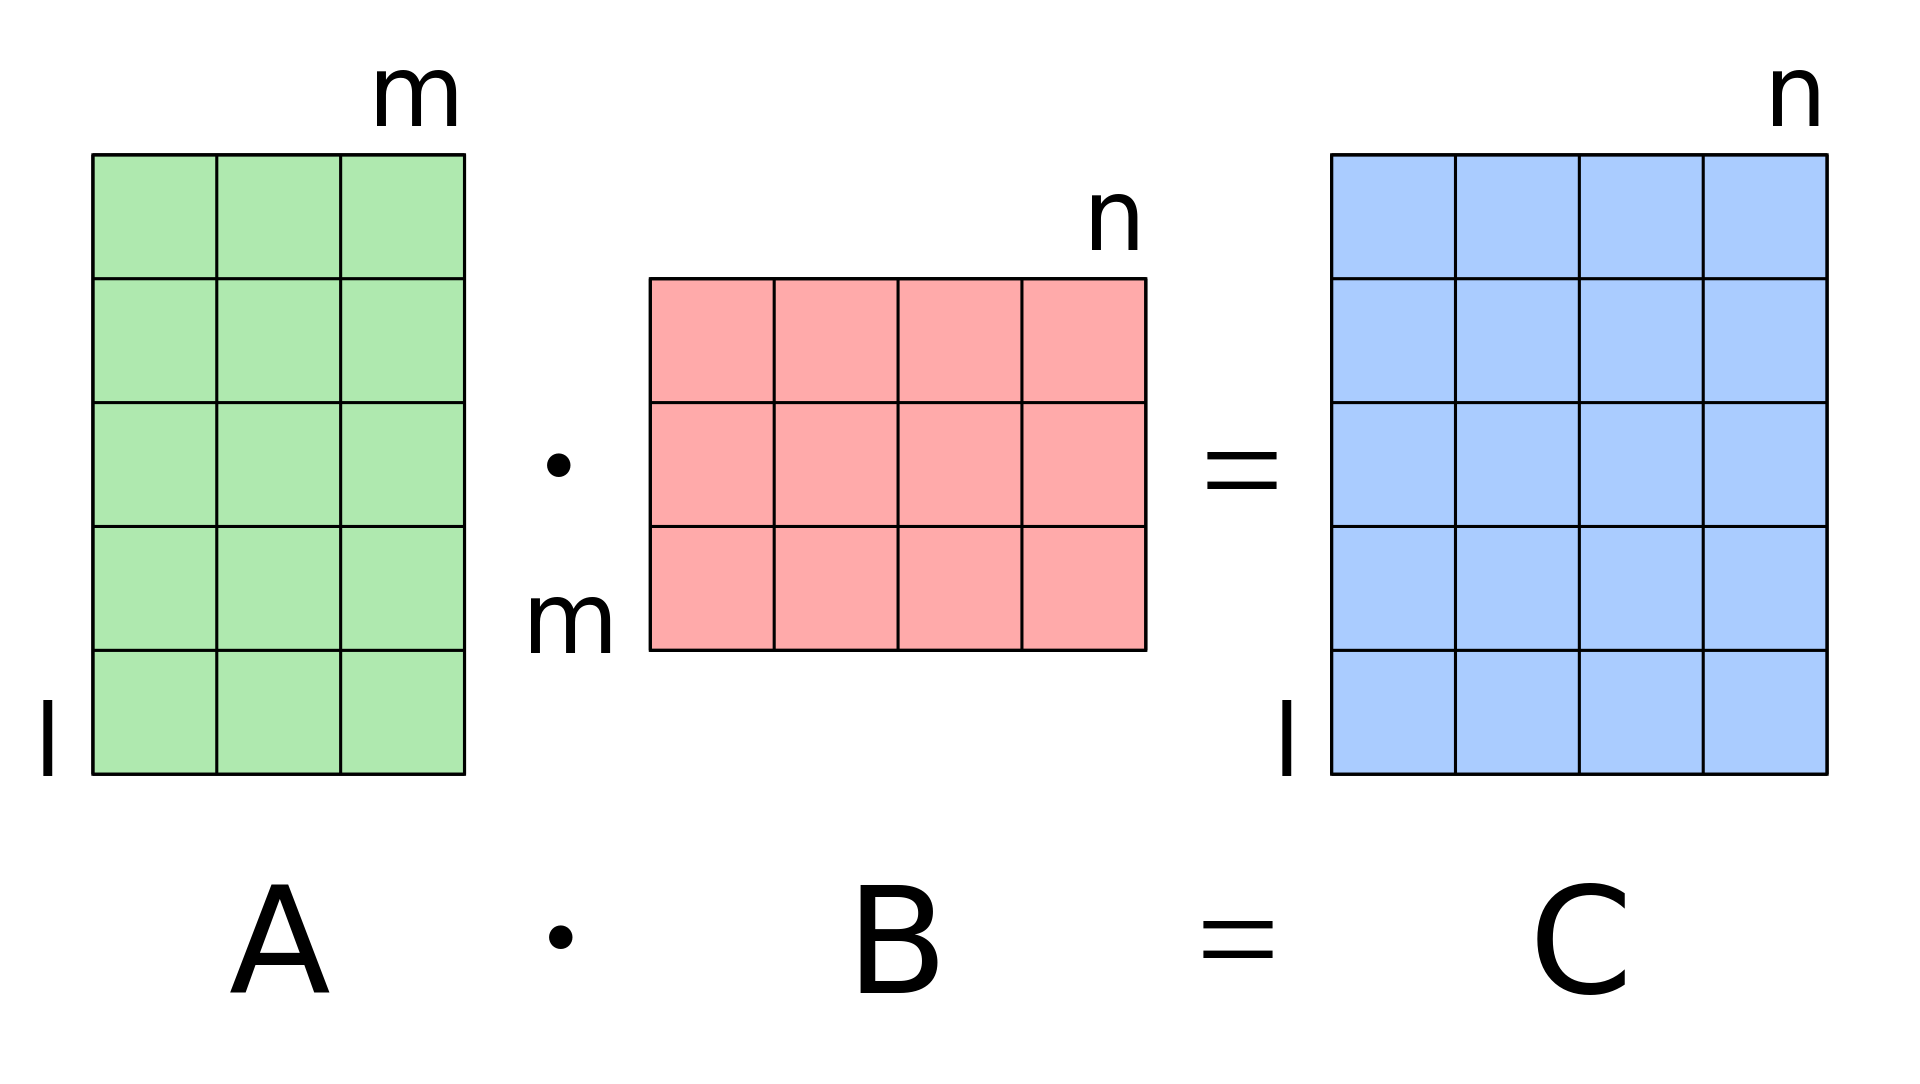
\includegraphics[width=0.5\textwidth,height=\textheight]{diplomka obrazky/4a.png}
\caption{Transformácia dimenzie matice pri násobení.}
\source{Zdroj: Prevzaté z [9].}
\end{center}
\end{figure}

Pri násobení matice skalárom, aka. jedným číslom, použijeme ako operátor
klasickú hviezdičku. Každý prvok matice bude prenásobený určeným číslom.

\begin{Shaded}
\begin{Highlighting}[]
\NormalTok{matica_riadky }\OperatorTok{*}\StringTok{ }\DecValTok{5}
\end{Highlighting}
\end{Shaded}

\begin{verbatim}
##         [,1] [,2] [,3]
## vektor1    5   10   15
## vektor2   20   25   30
## vektor3   35   40   45
\end{verbatim}

~

Pri násobení dvoch matíc sa používa trocha netradičný operátor
\(\%*\%\).

\begin{Shaded}
\begin{Highlighting}[]
\NormalTok{matica_riadky }\OperatorTok\StringTok{ }\NormalTok{matica_stlpce}
\end{Highlighting}
\end{Shaded}

\begin{verbatim}
##         vektor1 vektor2 vektor3
## vektor1      14      32      50
## vektor2      32      77     122
## vektor3      50     122     194
\end{verbatim}

~

Sčítanie matíc.

\begin{Shaded}
\begin{Highlighting}[]
\NormalTok{matica_riadky }\OperatorTok{+}\StringTok{ }\NormalTok{matica_stlpce}
\end{Highlighting}
\end{Shaded}

\begin{verbatim}
##         [,1] [,2] [,3]
## vektor1    2    6   10
## vektor2    6   10   14
## vektor3   10   14   18
\end{verbatim}

\hypertarget{transpozuxedcia-matice}{%
\subsubsection{Transpozícia matice}\label{transpozuxedcia-matice}}

Transponovaním matice dôjde k vzájomnej výmene riadkov a stĺpcov matice.
Takúto maticu označujeme ako \(A^T\). Ak bola prvotná matica \((m, n)\),
po transpozícií vznikne matica s rozmermi \((n, m)\). V R-ku matice
transponujeme pomocou funkcie \(t()\) ako \(transpose\).

\begin{Shaded}
\begin{Highlighting}[]
\NormalTok{matica_riadky}
\end{Highlighting}
\end{Shaded}

\begin{verbatim}
##         [,1] [,2] [,3]
## vektor1    1    2    3
## vektor2    4    5    6
## vektor3    7    8    9
\end{verbatim}

\begin{Shaded}
\begin{Highlighting}[]
\KeywordTok{t}\NormalTok{(matica_riadky)}
\end{Highlighting}
\end{Shaded}

\begin{verbatim}
##      vektor1 vektor2 vektor3
## [1,]       1       4       7
## [2,]       2       5       8
## [3,]       3       6       9
\end{verbatim}

\hypertarget{hodnosux165-rank-matice}{%
\subsubsection{Hodnosť (rank) matice}\label{hodnosux165-rank-matice}}

V zadaniach od vás bude požadované vyrátať hodnosť matice, čo sa zvykne
označovať aj ako rank matice. Hodnosť matice je maximálny počet lineárne
nezávislých riadkov, alebo stĺpcov, v matici. Dva vektory \textbf{a}, \textbf{b} nazývame
lineárne závislé vektory práve vtedy, ak existuje reálne číslo \(k\)
také, že platí:
\begin{align*}
\textbf{b} = k  \textbf{a}
\end{align*}

Ak táto rovnosť neplatí, vektory sú lineárne nezávislé. Keď sme
spomínali maximálny počet buď riadkov alebo stĺpcov, mysleli sme tým, že
ak nepracujeme so štvorcovou maticou, maximálna hodnosť môže byť najviac
rovná tomu, čoho je menej. Ak máme maticu 3x4, jej maximálna hodnosť
môže byť 3. Lebo riadkov máme menej. Ak by sme mali maticu 4x2,
maximálna hodnosť môže byť 2. Hodnosť matice sa v R-ku vyráta pomocou
funkcie \(qr()\).

\begin{Shaded}
\begin{Highlighting}[]
\CommentTok{# Predpokladajme, že pracujeme so štvorcovou maticou.}
\CommentTok{# Ak by ste mali overiť, či sú vektory lineárne nezávislé,}
\CommentTok{# všetky ich spojíme do matice, a vyrátame rank matice. Ak bude rank}
\CommentTok{# rovný počtu vektorov, vektory sú navzájom  lineárne nezávislé.}

\NormalTok{vektor1 <-}\StringTok{ }\KeywordTok{c}\NormalTok{(}\DecValTok{2}\NormalTok{, }\DecValTok{3}\NormalTok{, }\DecValTok{1}\NormalTok{, }\DecValTok{9}\NormalTok{)}
\NormalTok{vektor2 <-}\StringTok{ }\KeywordTok{c}\NormalTok{(}\DecValTok{1}\NormalTok{, }\DecValTok{0}\NormalTok{, }\DecValTok{3}\NormalTok{, }\DecValTok{4}\NormalTok{)}
\NormalTok{vektor3 <-}\StringTok{ }\KeywordTok{c}\NormalTok{(}\DecValTok{2}\NormalTok{, }\DecValTok{9}\NormalTok{, }\DecValTok{0}\NormalTok{, }\DecValTok{3}\NormalTok{)}
\NormalTok{vektor4 <-}\StringTok{ }\KeywordTok{c}\NormalTok{(}\DecValTok{4}\NormalTok{, }\DecValTok{7}\NormalTok{, }\DecValTok{2}\NormalTok{, }\DecValTok{4}\NormalTok{)}

\NormalTok{matica <-}\StringTok{ }\KeywordTok{rbind}\NormalTok{(vektor1, vektor2, vektor3, vektor4)}

\CommentTok{# Operátor $ dokáže extrahovať konkrétnu hodnotu, ktorú chceme}
\CommentTok{# extrahovať. Skúste použiť príkaz "qr(matica)", ktorý nám vyráta}
\CommentTok{# ešte pár ďalších vecí. Nás však zaujíma iba rank.}

\KeywordTok{qr}\NormalTok{(matica)}\OperatorTok{$}\NormalTok{rank }\CommentTok{# vyrátame hodnosť matice}
\end{Highlighting}
\end{Shaded}

\begin{verbatim}
## [1] 4
\end{verbatim}

\begin{Shaded}
\begin{Highlighting}[]
\CommentTok{# Vidíme, že rank je rovný počtu riadkov/stĺpcov, teda naše vektory}
\CommentTok{# sú lineárne nezávislé.}
\end{Highlighting}
\end{Shaded}

\hypertarget{determinant-matice}{%
\subsubsection{Determinant matice}\label{determinant-matice}}

Determinant matice si môžeme predstaviť ako hodnotu, ktorá je priradená
matici podľa toho, ako vyzerá. Matice môžu mať determinant nulový alebo
nenulový. Mohli by sme to rátať ručne, necháme to však R-ko vyrátať za
nás. Nás budú zaujímať aké vlastnosti sa s determinantom spájajú.

\begin{Shaded}
\begin{Highlighting}[]
\CommentTok{# Determinant môžeme vyrátať pomocou funkcie det().}
\end{Highlighting}
\end{Shaded}

\hypertarget{inverznuxe1-matica}{%
\subsubsection{Inverzná matica}\label{inverznuxe1-matica}}

Inverzná matica je matica \(A^{-1}\), ktorá nám po vynásobení pôvodnou
maticou A, dá jednotkovú maticu. Funguje to aj naopak, teda platí vzťah:

\[A * A^{-1} = A^{-1} * A = E\]

Inverznú maticu vytvoríme pomocou funkcie \(solve()\)

\hypertarget{singuluxe1rna-reguluxe1rna-matica}{%
\subsubsection{Singulárna / Regulárna
matica}\label{singuluxe1rna-reguluxe1rna-matica}}

Ak je matica regulárna, znamená to, že má inverziu. Ak je singulárna,
nemá inverziu, teda \(A^{-1}\) neexistuje.

\begin{itemize}
\tightlist
\item
  Matica je singulárna ak:

  \begin{itemize}
  \tightlist
  \item
    má determinant rovný nule,
  \item
    sa hodnost nerovná poctu riadkov (ak má napr. 3x3 matica hodnost 2)
  \end{itemize}
\item
  Matica je regulárna ak:

  \begin{itemize}
  \tightlist
  \item
    má nenulový determinant,
  \item
    sa hodnost rovná poctu riadkov/stlpcov.
  \end{itemize}
\end{itemize}

\newpage

\hypertarget{pruxe1ca-s-datasetmi-a-ich-analuxfdza}{%
\section{Práca s datasetmi a ich
analýza}\label{pruxe1ca-s-datasetmi-a-ich-analuxfdza}}

Vrhneme sa na:

\begin{itemize}
\tightlist
\item
  načítanie datasetov do R-ka a objektov,
\item
  manipuláciu datasetov,
\item
  vysvetlenie lineárneho regresného modelu,
\item
  prácu s regresnými modelmi.
\end{itemize}

\hypertarget{naux10duxedtanie-duxe1t}{%
\subsection{Načítanie dát}\label{naux10duxedtanie-duxe1t}}

Načítať dáta je možné rôznymi spôsobmi. V okne \(Environment\) môžete
kliknúť na \(Import \ dataset\) a vybrať typ súboru, aký chcete
importovať. Sofistikovanejšie je však načítavanie údajov pomocou
funkcií. Tých je tiež niekoľko, plus, existujú rôzne balíky, ktoré sú
vyvinuté na zlepšenie práce s dátami a ich vizáže. Vám však bude stačíť
jediná funkcia a to \(read.csv2\). Predtým než funkciu použijeme, si
však treba nastoliť isté štandardy. Ideálne je, aby ste mali vytvorenú
zložku, v ktorej budete mať všetky datasety (excelovské súbory) a pekne
oddelené zložky k cvičeniam. Nazývame to ``working directory'' AKA
pracovný adresár. Na zistenie, kde je Váš momentálny pracovný adresár
použijeme funkciu \(getwd()\) (get working directorty). Potrebujeme to
vedieť preto, lebo do funkcie \(read.csv2\) potrebujeme zadať argument
umiestnenia súboru. A je ľahšie zadať:

\begin{Shaded}
\begin{Highlighting}[]
\KeywordTok{read.csv2}\NormalTok{(}\StringTok{"udaje_o_pocte_kaciatok"}\NormalTok{)}
\CommentTok{# než}
\KeywordTok{read.csv2}\NormalTok{(}\StringTok{"C:/Desktop/MilanRozok/ekonometria/udaje_o_pocte_kaciatok.csv"}\NormalTok{)}
\end{Highlighting}
\end{Shaded}

Určenie nového adresára je možné urobiť pomocou \(setwd()\) (set working
directory), kde ako argument zadáme cestu do nového adresára, avšak,
jednoduchšie je kliknúť vľavo hore na:

\begin{center}

Session -\textgreater{} Set Working Directory -\textgreater{} Choose
directory,

\end{center}

a vybrať si adresár manuálne. Všetky datasety potom môžeme načítať
funkciou \(read.csv2()\) už len pomocou uvedenia názvu v úvodzovách, a
nemusíme uvádzať celú cestu umiestnenia súboru.

\hypertarget{read.csv2}{%
\subsubsection{read.csv2()}\label{read.csv2}}

Súbory typu .CSV znamenajú doslovne \(Comma-separated \ values\), teda
hodnoty oddelené čiarkami. Keď sa bavíme o formáte .CSV predstavte si
súbor, kde každá hodnota má svoj riadok, a každá premenná má svoj
stĺpec. Ako hodnoty sa chápe oddelenie stlpcov, teda stĺpce sú väčšinou
oddelené čiarkami. To je však taký teoretický prístup, v praxi môžu byť
tieto hodnoty oddelené aj inými spôsobmi. Hlavné však je pozerať na
koncovku súboru, resp. súbor (napr. z Excelu), uložiť ako .CSV súbor.
Funkcie \(read.csv()\) a \(read.csv2()\) robia to isté, jediné v čom sa
líšia je ich defaultné nastavenie. \(read.csv()\) ráta, že sa na
oddelenie desatinných miest používa bodka (čo je také americké), a
\(read.csv2()\), používa na oddelenie desatinných miest čiarku (čo je
také európske). To je dôvod, prečo primárne používame \(read.csv2()\).

\hypertarget{pruxe1ca-so-vstavanuxfdmi-datasetmi}{%
\subsubsection{Práca so vstavanými
datasetmi}\label{pruxe1ca-so-vstavanuxfdmi-datasetmi}}

R-ko obsahuje vstavané datasety, ktoré si môžeme všetky vypísať pomocou:

\begin{Shaded}
\begin{Highlighting}[]
\KeywordTok{data}\NormalTok{()}
\end{Highlighting}
\end{Shaded}

V tomto sprievodcovi budeme pracovať s dátami, ktoré si môžete načítať
zo vstavaného balíka \(datasets\). Je to z dôvodu, že je to proste
jednoduché. Na hodinách budete pracovať s pravými ekonomickými
datasetmi, avšak pre ukážku, ako čo funguje, a ako s čím súvisí nám
postačia základné datasety, ktoré sú ľahké na pochopenie. Ak si budete
chcieť overiť nejakú funkciu či teóriu, budete si môcť za pochodu
načítať dataset, s ktorým ste oboznámený, a otestovať, čo potrebujete.

\begin{Shaded}
\begin{Highlighting}[]
\CommentTok{# Pre načítanie datasetu do objektu použijeme trocha nezvyčajný prístup,}
\CommentTok{# kde "datasets" predstavuje názov balíku, a "mtcars" dataset, ktorý}
\CommentTok{# chceme sprístupniť.}
\CommentTok{# Pomocou "::" sprístupníme konkrétny objekt z balíka.}
\NormalTok{data <-}\StringTok{ }\NormalTok{datasets}\OperatorTok{::}\NormalTok{mtcars}
\CommentTok{# Ak by sme datasetu nechceli priradiť vlastný názov,}
\CommentTok{# ale ponechať originálny:}
\KeywordTok{data}\NormalTok{(}\StringTok{"mtcars"}\NormalTok{)}
\CommentTok{# Funkcia bude fungovať aj bez úvodzoviek.}
\end{Highlighting}
\end{Shaded}

\newpage

\hypertarget{jednoduchuxe1-lineuxe1rna-regresia}{%
\section{Jednoduchá lineárna
regresia}\label{jednoduchuxe1-lineuxe1rna-regresia}}

Hlavným nástrojom ekonometrie je regresia. Cieľom regresie je zistiť ako
určená/é nezávislé premenné, ovplyvňujú jednu závislú premennú. Ak \(Y\)
je závislá a \(X\) nezávislá, tak regresujeme, robíme regresiu, Y na X.
Čo však tá magická skrinka vlastne robí?

\begin{Shaded}
\begin{Highlighting}[]
\CommentTok{# Predpokladajme, že máme načítaný dataset "mtcars".}
\CommentTok{# Pomocou funkcie "head()" si načítame prvých 6 riadkov.}
\CommentTok{# Alternatíva je "tail()" (ako chvost),}
\CommentTok{# čím vypíšeme posledných 6 riadkov.}

\KeywordTok{head}\NormalTok{(data)}
\end{Highlighting}
\end{Shaded}

\begin{verbatim}
##                    mpg cyl disp  hp drat    wt  qsec vs am gear carb
## Mazda RX4         21.0   6  160 110 3.90 2.620 16.46  0  1    4    4
## Mazda RX4 Wag     21.0   6  160 110 3.90 2.875 17.02  0  1    4    4
## Datsun 710        22.8   4  108  93 3.85 2.320 18.61  1  1    4    1
## Hornet 4 Drive    21.4   6  258 110 3.08 3.215 19.44  1  0    3    1
## Hornet Sportabout 18.7   8  360 175 3.15 3.440 17.02  0  0    3    2
## Valiant           18.1   6  225 105 2.76 3.460 20.22  1  0    3    1
\end{verbatim}

\begin{Shaded}
\begin{Highlighting}[]
\CommentTok{# Vidíme, že je to súbor aút, s rôznymi parametrami.}
\CommentTok{# My sa budeme snažiť vysvetliť vplyv "hp" (horsepower, konské sily), }
\CommentTok{# na "mph" (miles per galon, čiže koľko kilometrov má auto dojazd).}
\end{Highlighting}
\end{Shaded}

Pozrime sa na tento model:
\[y_i = \beta_0 + \beta{x_i} + \epsilon_i.\]

Jedná sa o základný model lineárnej regresie. Ak si bety predstavíme ako
obyčajné hodnoty, model v tomto jednoduchom znení by Vám z matematiky
mohol byť povedomý. Výsledkom modelu je priamka \(y\), kde \(\beta_0\)
je obyčajná hodnota v ktorej je os Y pretnutá, \(\beta_1\) určuje sklon
priamky. Keďže priamka nebude prechádzať každou nameranou hodnotou,
\(\epsilon\) v modeli znázorňuje tento priestor medzi meraniami a
priamkou. Označujeme ho ako náhodnú zložku. Môže byť spôsobená mnohými
spôsobmi. Okrem iného napríklad: chybným meraním, náhodou, alebo
premennými, ktoré sme do modelu nezahrnuli. Jedno auto so 150 koňskými
silami môže na plnú nádrž prejsť 500km a druhé len 350. Môže to byť
spôsobené váhou, avšak v modeli máme len výkon auta. Táto zložka sa v
priemere rovná nule, a z modelu nám odpadne (viac o tom neskôr). Tento
model si môžeme v našom príklade prepísať ako:
\[mpg_i = \beta_0 + \beta_1{hp_i} + \epsilon_i.\] Priamka, ktorá by
vznikla výsledkom tohto modelu sa nazýva populačná regresná priamka. Na
vyhodnotenie takéhoto modelu by sme však potrebovali dáta z celej
určenej populácie, čo je veľmi často prakticky nemožné. Vo všeobecnosti
sú populačné parametre \(\beta_0\) a \(\beta_1\) neznáme. Avšak dokážeme
ich odhadnúť pomocou estimátorov. Preto pracujeme so vzorkami, ktoré
dokážeme reálne odpozorovať a zozbierať. Estimátory zo vzorky dokážu
poskytnúť dostatočne dôveryhodné odhady koeficientu v populácií. Poďme
si to teda ukázať na našej vzorke.

Skúsme si hodiť do grafu výkon a dojazd, nech sa pozrieme na vzťah medzi
týmito premennými.

\begin{Shaded}
\begin{Highlighting}[]
\CommentTok{# Plotneme si dáta, ktoré dáme do regresie, čiže "mpg" a "hp".}

\KeywordTok{plot}\NormalTok{(}\DataTypeTok{x =}\NormalTok{ data}\OperatorTok{$}\NormalTok{hp, }\DataTypeTok{y =}\NormalTok{ data}\OperatorTok{$}\NormalTok{mpg, }\DataTypeTok{ylab =} \StringTok{"ylab ako y label"}\NormalTok{, }
     \DataTypeTok{xlab =} \StringTok{"tu máme výkon",} \StringTok{main = "}\NormalTok{Vzťah dojazdu a výkonu motora}\StringTok{")}
\end{Highlighting}
\end{Shaded}

\begin{figure}
\begin{center}
    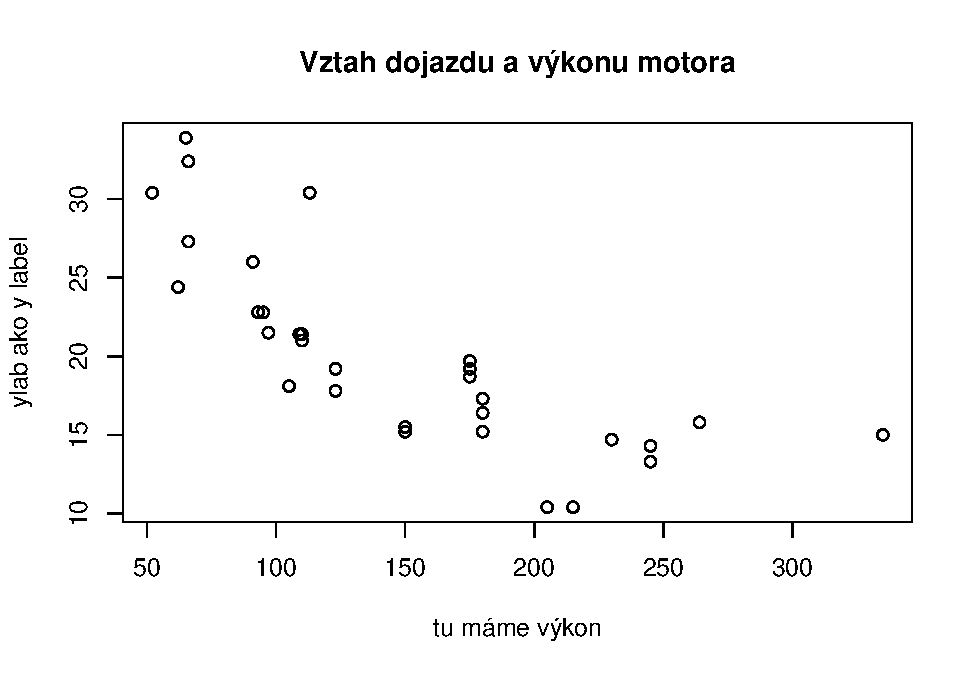
\includegraphics[width=0.8\textwidth,height=\textheight]{test_files/figure-latex/unnamed-chunk-39-1.pdf}
    \caption{Výstup funkcie plot().}
    \source{Zdroj: Vlastná tvorba.}
\end{center}
\end{figure}

\newpage

Vidíme istú negatívnu závislosť. Chceli by sme si to však potvrdiť
číslami. Bolo by fajn napasovať medzi tieto pozorovania takú priamku,
ktorá bude ku každému pozorovaniu čo najbližšie. Keďže nepoznáme
parametre populácie, budeme pracovať s ich estimátormi, odhadcami.
Estimátory označíme striežkou ako \(\hat\beta_0{}\) a \(\hat\beta_1{}\).
Model bude vyzerať následovne:
\[\hat{mpg_i} = \hat\beta_0 + \hat \beta_1{hp_i}.\] \textgreater{}
\textbf{Náhodná zložka (error term) vypadne, lebo jej očakávaná hodnota
sa rovná nule.}

Skúsme si takýto model zostrojiť v R-ku, a priamku dopasovať do grafu.

\begin{Shaded}
\begin{Highlighting}[]
\CommentTok{# Chceme zistiť dopad "hp" na "mpg".}
\CommentTok{# Použijeme funkciu "lm()", ako linear model.}
\CommentTok{# Na konci musíme ako argument uviesť dáta, ktoré použijeme.}

\NormalTok{model <-}\StringTok{ }\KeywordTok{lm}\NormalTok{(mpg }\OperatorTok{~}\StringTok{ }\NormalTok{hp, }\DataTypeTok{data =}\NormalTok{ data)}

\CommentTok{# Alternatívne môžeme model napísať pomocou extrakcie takto.}
\CommentTok{# Preferujem tento postup.}

\NormalTok{model <-}\StringTok{ }\KeywordTok{lm}\NormalTok{(data}\OperatorTok{$}\NormalTok{mpg }\OperatorTok{~}\StringTok{ }\NormalTok{data}\OperatorTok{$}\NormalTok{hp)}

\CommentTok{# Dostaneme dva koeficienty.}
\CommentTok{# Jeden pre intercept Beta0, a druhý pre Beta1 ako "hp".}

\NormalTok{model}
\end{Highlighting}
\end{Shaded}

\begin{verbatim}
## 
## Call:
## lm(formula = data$mpg ~ data$hp)
## 
## Coefficients:
## (Intercept)      data$hp  
##    30.09886     -0.06823
\end{verbatim}

\begin{Shaded}
\begin{Highlighting}[]
\CommentTok{# Intercept sa väčšinou neinterpretuje, slúži len pre určenie}
\CommentTok{# počiatočnej hodnoty. Ak by sme koeficient interpretovali,}
\CommentTok{# mohli by sme povedať, že auto s nula koňmi prejde 30 míľ na galón.}
\CommentTok{# Koeficient B1 by sme interpretovali ako:}
\CommentTok{# "každá extra konská sila, zníži dojazd o -0.068 míle".}
\end{Highlighting}
\end{Shaded}

\begin{Shaded}
\begin{Highlighting}[]
\CommentTok{# Znova si plotneme dáta.}
\KeywordTok{plot}\NormalTok{(}\DataTypeTok{x =}\NormalTok{ data}\OperatorTok{$}\NormalTok{hp, }\DataTypeTok{y =}\NormalTok{ data}\OperatorTok{$}\NormalTok{mpg, }\DataTypeTok{ylab =} \StringTok{"Dojazd"}\NormalTok{, }\DataTypeTok{xlab =} \StringTok{"Výkon",}
\StringTok{     main = "}\NormalTok{Vzťah dojazdu a výkonu motora}\StringTok{")}

\StringTok{# A pomocou funkcie "}\KeywordTok{abline}\NormalTok{()}\StringTok{" napasujeme do grafu priamku modelu.}
\StringTok{# Abline ako priamka z bodu A do bodu B.}

\StringTok{abline(model) }
\end{Highlighting}
\end{Shaded}

\begin{figure}
\begin{center}
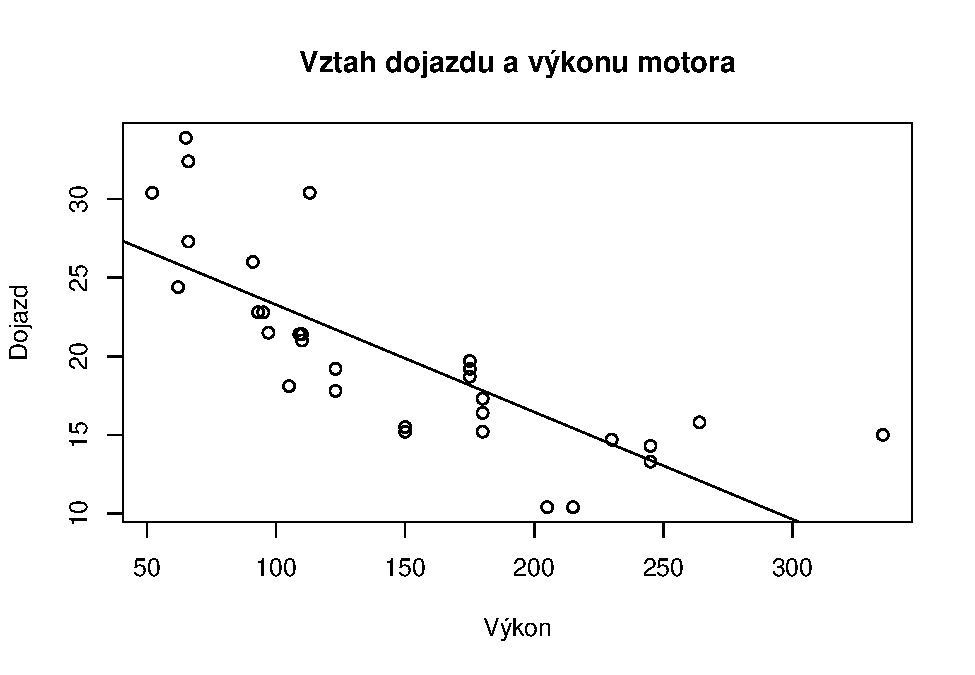
\includegraphics[width=0.8\textwidth,height=\textheight]{test_files/figure-latex/unnamed-chunk-41-1.pdf}
\caption{Výstup funkcie plot().}
\source{Zdroj: Vlastná tvorba.}
\end{center}
\end{figure}

Z grafu pozorujeme, že aj tu priamka neprechádza všetkými pozorovaniami,
túto kolmú vzdialenosť medzi priamkou a každým pozorovaním označíme ako
\(\hat{u}\). V tomto modeli to neoznačuje odhad náhodnej zložky
\(\epsilon\), ale výpočtovú nepresnosť modelu. Môžeme to brať ako takého
súrodenca k náhodnej zložke. Obe chyby predstavujú podobnú vec,
vzdialenosť medzi priamkou a pozorovaním. Priamku populácie je však
neznáma, teda aj táto vzdialenosť \(\epsilon\) je neznáma. Na druhú
stranu, zvyšky \(\hat{u}\) sú vyrátané z dát, a dokážeme ich presne
zmerať. Ako však vyrátame bety? Iste ste už začuli o OLS, teda Ordinary
Least Squares alebo Metódy najmenších štvorcov. Bety so striežkou
nazývame ako OLS estimátory. Metóda najmenších štvorcov sa to volá
preto, lebo vezmeme zvyšky \(\hat{u}\) z modelu, umocníme ich na druhú
mocninu (urobíme z nich štvorce), a minimalizujeme ich. Osobne si
nemyslím, že v tomto štádiu vašej výučby má veľký význam sústrediť sa na
odvodenie týchto estimátorov. Osobne mi to moc nedalo, preto sa skôr
zameriame na výsledky týchto odvodzovaní, nech nadobudneme trocha
intuície. Vysvetlíme si graficky, čo touto metódou chceme docieliť.

\begin{figure}
\begin{center}
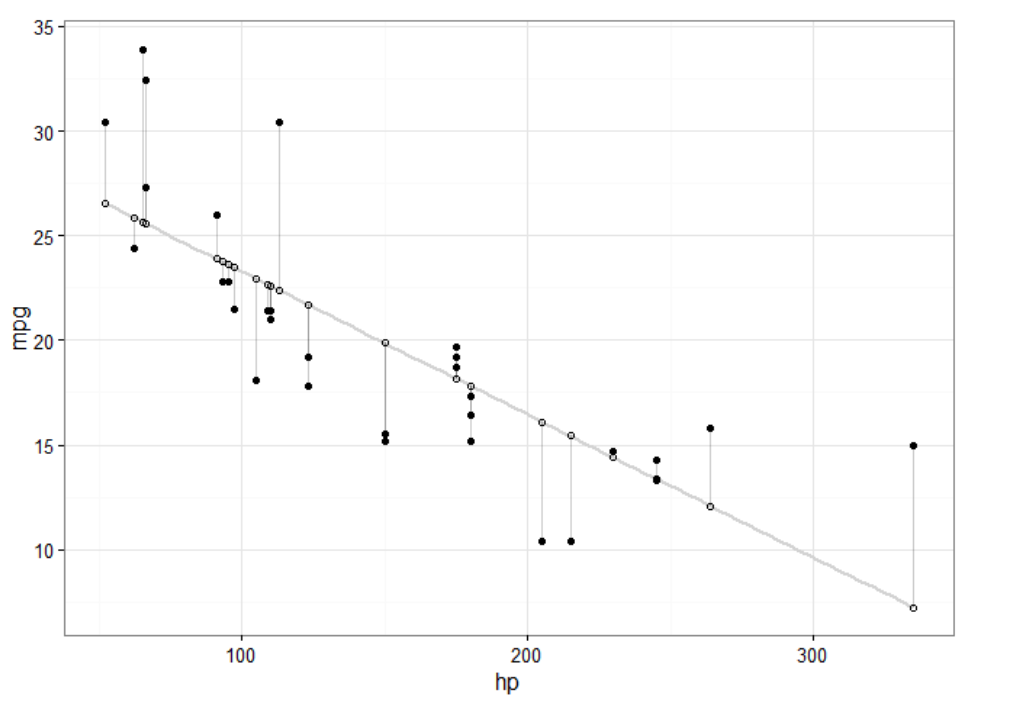
\includegraphics[width=0.8\textwidth,height=\textheight]{diplomka obrazky/4.png}
\caption{Vyobrazenie vzdialenosti rezíduí k priamke.}
\source{Zdroj: Prevzaté z [10].}
\end{center}
\end{figure}

Tieto vzdialeností predstavujú naše ``residuals'' \(\hat{u}_i\), naše
zvyšky z modelu, naše nepresnosti. Každý data point má svoj zvyšok.
Logicky chceme, aby priamka čo najtesnejšie vystihovala dáta, chceme tým
pádom čo najviac zmenšiť zvyšky. Poďme sa k tým zvyškom dopracovať.

Pozorovanie sa rovná bodu na priamke \(\hat\beta_0 + \hat\beta{x}_i\)
plus zvyšok \(\hat{u}_i\):
\[ y_i = \hat\beta_0 + \hat\beta{x}_i + \hat{u}_i.\]

\begin{center}

Poprehadzujme si to, nech máme na jednej strane zvyšok \(\hat{u}_i\):

\end{center}
\[ \hat{u}_i = y_i - \hat\beta_0 - \hat\beta{x}_i.\]

Väčšinou narazíme na takýto zápis zvyškov, a to rozdiel medzi
pozorovanou hodnotou a odhadnutou hodnotou na priamke:
\[\hat{u}_i = y_i - \hat{y_i}.\]

\begin{center}

a keďže
\end{center}
\[ \hat{y}_i =\hat\beta_0 + \hat\beta{x}_i,\]

Tak sme tam, kde sme boli na začiatku, keď sme si dali zvyšok
\(\hat{u}_i\) na jednu stranu. OLS metóda urobí to, že minimalizuje
súčet našich umocnených zvyškov \(\hat{u}_i\):
\[min\sum (y_i - \hat\beta_0 - \hat\beta_1{x}_i)^2.\]

Tým, že minimalizujeme zvyšky dostaneme čo najlepšiu priamku, ktorá bude
sedieť čo najtesnejšie s dátami. Táto minimalizácia nám poskytne vzorec
na výpočet OLS estimátorov. Estimátorov parametrov populácie. Bavíme sa
o odhadcoch priesečníka, \(\beta_0\), a sklonu, \(\beta_1\). A keď sa
bavíme o odhadcoch, píšeme ich ako \(\hat\beta_0\) a \(\hat\beta_1\).
Nech si pamätáte.

Na hodinách sa stretnete so vzorcom pre výpočet biet v maticovej forme.
A to:
\[Est(\beta) = \hat\beta = (X^TX)^{-1}X^Ty.\]

\begin{quote}
\emph{T-čka znamenajú transpose matice a -1 vyrátanie inverzie.}
\end{quote}

\begin{Shaded}
\begin{Highlighting}[]
\CommentTok{# Inverznu maticu vyrátame pomocou "solve()" a}
\CommentTok{# transpozíciu pomocou "t()".}
\CommentTok{# V R-ku by sme to vyrátali ako:}

\KeywordTok{solve}\NormalTok{(}\KeywordTok{t}\NormalTok{(X) }\OperatorTok\StringTok{ }\NormalTok{X) }\OperatorTok\StringTok{ }\KeywordTok{t}\NormalTok{(X) }\OperatorTok\StringTok{ }\NormalTok{y}\ErrorTok{)}
\end{Highlighting}
\end{Shaded}

Tento vzorec by som nazval funkčným, avšak určite nie intuitívnym.
Pracujete s ním preto, lebo:

\begin{itemize}
\tightlist
\item
  takáto forma je ľahšie spracovateľná pre výpočtovú techniku,
\item
  R-ko pri práci s datasetom ho aj tak pretvorí na maticu, predtým než
  podá výsledky,
\item
  tento vzorec funguje ako pre jednoduchú lineárnu regresiu (jedno Y a
  jedno X), tak aj pre viacnásobnú regresiu (jedno Y a viacero X).
\end{itemize}

Ono, R-ko to urobí všetko za Vás, samo vyráta všetky koeficienty, nuž
nechceli by ste vedieť, čo tá \(\hat\beta\) vlastne robí? Pri
jednoduchej lineárnej regresií dokážeme OLS beta estimátory zapísať aj
takto:
\[\hat\beta_0 = \overline{y} - (\hat\beta_1\overline{x})\]

\[\hat\beta_1 = \frac{\sum_{i=1}^{n} (x_i - \overline{x})(y_i - \overline{y})}{\sum_{i=1}^{n} (x_i - \overline{x})^2}\]


\begin{quote}
\emph{Čiara nad písmenom znamená priemer, teda ybar(takto to čítame) je
priemer všetkých hodnôt ``y'' v datasete.}
\end{quote}

Neopúšťajte ma. Ak Vám tento vzorec nie je povedomý, nič sa nedeje.
Pozrieme sa na to. Rozdeľme si to na vrch a spodok. Začneme menovateľom,
lebo je kratší, hm.

Súčet od i = 1 po n znamená, že vykonáme operáciu pre každé \(x\) v
datasete a výsledky operácií sčítame.


\begin{quote}
\begin{center}
\emph{Summation znak sa nazýva grécky sigma.}
\end{center}
\end{quote}


Od každého \(x\) odčítame priemernú hodnotu \(\overline{x}\) a umocníme
to. Získame tým variabilitu okolo priemeru, inak povedané, ako veľmi sú
data v datasete rozptýlené. Dostaneme rozptyl. Je dôležité podotknúť, že
rozptyl kvôli umocneniu nikdy nebude záporný. Dôležité je to preto, lebo
vzťah v čitateli určuje, či je \(\beta\) pozitívna alebo negatívna.
Takže menovateľ neovplyvní kladnosť či zápornosť čitateľa.

Vzťah v čitateli vyzerá celkom podobne k tomu v menovateli, hm? A nie je
to náhoda. Vzťah v čitateli je obyčajná kovariancia, inak povedané,
spoločný rozptyl. Predstavuje závislosť medzi dvoma veličinami. Tento
vzťah neumocňujeme, pretože chceme vidieť, či bude závislosť pozitívna,
alebo negatívna.

\begin{quote}
\emph{Kovariancia či korelácia? Čo je čo? Korelácia je štandardizovaná
kovariancia. Obe vysvetľujú to isté, líšia sa len v rozsahu. Kovarianciu
predelíme násobkom smerodajných odchýlok x a y, a získame koreláciu.
Štandardizujeme to preto, aby sme sa vedeli orientovať, aký veľký je v
skutočnosti vzťah medzi premennými. Ak sa bavíme o kovariancii hmotnosti
v kilogramoch a dĺžky lietadla v metroch, výsledné hodnoty budú veľmi
vysoké. Ak budú kladné, budeme vedieť, že je medzi nimi lineárna
závislosť, ale nevieme aká veľká. Ak by sme porovnávali kovarianciu
kurzu EUR a USD, výsledné hodnoty budú síce menšie, ale stále o nič viac
vhodné na interpretovanie. Ak však tieto hodnoty predelíme násobkom
smerodajných odchýlok, teda ich štandardizujeme, výsledné hodnoty budú
porovnateľné pre akékoľvek premenné. Keďže ťažké a dlhé lietadlo bude
mať úmerne veľké smerodajné odchýlky, kdežto výmenný kurz bude mať
smerodajnú odchýlku prislúchajúcu hodnotám kurzu. Hodnoty v korelácií
budú spadať medzi hranice -1 a 1. Kde záporná hodnota predstavuje
negatívnu lineárnu závislosť, a naopak.}
\end{quote}

Pri odhade však nechceme hodnoty štandardizovať, ale vecne odhadnúť
použiteľné hodnoty koeficientov. \(\hat\beta_1\) si jednoducho zapíšeme
ako:

\[\hat\beta_1 = \frac{Cov(x, y)}{Var(x)}.\] Otestujme si, či to naozaj
funguje.

\begin{Shaded}
\begin{Highlighting}[]
\CommentTok{# Pripomeňme si hodnoty nášho modelu.}
\NormalTok{model}
\end{Highlighting}
\end{Shaded}

\begin{verbatim}
## 
## Call:
## lm(formula = data$mpg ~ data$hp)
## 
## Coefficients:
## (Intercept)      data$hp  
##    30.09886     -0.06823
\end{verbatim}

\begin{Shaded}
\begin{Highlighting}[]
\CommentTok{# Na poradí pri kovariancii nezáleží.}
\NormalTok{kovar <-}\StringTok{ }\KeywordTok{cov}\NormalTok{(data}\OperatorTok{$}\NormalTok{mpg, data}\OperatorTok{$}\NormalTok{hp)}

\NormalTok{rozptyl <-}\StringTok{ }\KeywordTok{var}\NormalTok{(data}\OperatorTok{$}\NormalTok{hp)}
\NormalTok{beta1 <-}\StringTok{ }\NormalTok{kovar}\OperatorTok{/}\NormalTok{rozptyl}

\KeywordTok{print}\NormalTok{(beta1)}
\end{Highlighting}
\end{Shaded}

\begin{verbatim}
## [1] -0.06822828
\end{verbatim}

\begin{Shaded}
\begin{Highlighting}[]
\CommentTok{# Oba parametre majú hodnotu -0.068 a rovnajú sa.}
\CommentTok{# Skúsme B0.}

\NormalTok{ybar <-}\StringTok{ }\KeywordTok{mean}\NormalTok{(data}\OperatorTok{$}\NormalTok{mpg)}
\NormalTok{xbar <-}\StringTok{ }\KeywordTok{mean}\NormalTok{(data}\OperatorTok{$}\NormalTok{hp)}

\NormalTok{beta0 <-}\StringTok{ }\NormalTok{ybar }\OperatorTok{-}\StringTok{ }\NormalTok{(beta1 }\OperatorTok{*}\StringTok{ }\NormalTok{xbar)}

\KeywordTok{print}\NormalTok{(beta0)}
\end{Highlighting}
\end{Shaded}

\begin{verbatim}
## [1] 30.09886
\end{verbatim}

\begin{Shaded}
\begin{Highlighting}[]
\CommentTok{# Sedí. :)}
\end{Highlighting}
\end{Shaded}

Nevravím, že sme objavili Ameriku, ale aspoň viete, že \(\hat\beta_0\)
je nejaký priemer \(y\) a od toho odčítame \(\hat\beta_1\) vynásobenú
priemerom \(x\). A neskrýva sa za tým žiaden ťažký imaginárny vzorec.
Taktiež, že \(\hat\beta_1\) je spoločný rozptyl závislej a nezávislej
premennej, vydelený rozptylom nezávislej premennej.

Ako však vieme, či estimátorom \(\hat\beta_0\) a \(\hat\beta_1\) môžeme
veriť?

\newpage

\hypertarget{trocha-ux161tatistiky}{%
\section{Trocha štatistiky}\label{trocha-ux161tatistiky}}

Predtým, než si povieme o podmienkach lineárnej regresie Vás oboznámim s
pár záležitosťami, s ktorými sa stretnete, a napriek tomu, že sú pomerne
jednoduché by Vám zabrali dosť googlenia.

Prejdeme si:

\begin{itemize}
\tightlist
\item
  normálne rozdelenie,
\item
  očakávanú hodnotu,
\item
  zákon veľkých čísel,
\item
  náhodný výber,
\item
  centrálnu limitnú vetu.
\end{itemize}

Možno ste si všimli, že pri interpretáciach koeficientov sa často
opakuje niečo v zmyysle:``V priemere nám pri zvýšeni bla bla bla
narastie o bla bla bla.'' To \textbf{v priemere} je veľmi podstatné.
Väčšinou pracujeme so vzorkami, ktoré boli zozbierané z populácie, ktorá
je pre nás neznáma. Ideálne boli vybrané náhodným výberom, čo spôsobí,
že pozorovania vo vzorke sú náhodnými veličinami, a štatistiky ktoré z
nich vyrátame sú taktiež náhodné veličiny. Prečo je to podstatné sa
dozvieme v nasledujúcich konceptoch.

\begin{quote}
\emph{Keď sa bavíme o štatistikách, máme na mysli akúkoľvek hodnotu,
ktorú je možné vyrátať a opisuje niečo. Priemer je štatistika, rozptyl
je štatistika."}
\end{quote}

\hypertarget{normuxe1lne-rozdelenie}{%
\subsection{Normálne rozdelenie}\label{normuxe1lne-rozdelenie}}

Je potrebné vedieť, ako toto rozdelenie vyzerá, a aké má vlastnosti,
keďže mnoho konceptov v štatistike, sa točí okolo tohto rozdelenia,
kvôli jeho sladkým vlastnostiam. Normálne rozdelenie je rozdelenie
pravdepodonosti, ktoré je symetrické okolo priemeru, čím znázorňuje, že
hodnoty okolo priemeru majú vyššiu pravdepodobnosť výskytu. V porovnaní
s dátami na chvoste rozdelenia. Normálne rozdelenie má dva parametre:

\begin{itemize}
\tightlist
\item
  priemer,
\item
  smerodajnú odchýlku.
\end{itemize}

Pre normálne rozdelenie platí, že 68\% pozorovaní je v rozmedzí 1
smerodajnej odchýlky (od priemeru na každú stranu jedna), 95\%
pozorovaní je v romedzí 2 smerdajných odchýlok a 99,7\% pozorovaní v
rozmedzí 3 smerodajných odchýlok. To sa nám zíde pri testovaní hypotéz.

\begin{Shaded}
\begin{Highlighting}[]
\CommentTok{# Zostrojme si pre ilustráciu normálne rozdelenie.}
\CommentTok{# Môžeme použiť dnorm(), pre vyrátanie krásneho normálneho rozdelenia,}
\CommentTok{# ktorému by sme zadali vlastné hodnoty, my však použijeme rnorm(),}
\CommentTok{# pre vygenerovanie n hodnôt z normálneho rozdelenia.}

\NormalTok{nrozdelenie <-}\StringTok{  }\KeywordTok{rnorm}\NormalTok{(}\DataTypeTok{n =} \DecValTok{1000}\NormalTok{, }\DataTypeTok{mean =} \DecValTok{20}\NormalTok{, }\DataTypeTok{sd =} \DecValTok{5}\NormalTok{)}

\CommentTok{# Použijeme hist() namiesto plot(). Funkcia plot() by defaultne použila}
\CommentTok{# scatterplot.}
\CommentTok{# Argument "breaks" určí, na koľko častí rozlámeme náš histogram.}
\CommentTok{# Viacej častí nám umožní krajšie vystihnúť normálne rozdelenie.}
\CommentTok{# Funkciou par() si zobrazíme dva grafy vedľa seba, a ukážeme rozdiel.}

\KeywordTok{par}\NormalTok{(}\DataTypeTok{mfrow=}\KeywordTok{c}\NormalTok{(}\DecValTok{1}\NormalTok{, }\DecValTok{2}\NormalTok{)) }

\CommentTok{# Všimnime si, že sú centrované okolo priemeru, ktorý sme zadali ako 20.}

\KeywordTok{hist}\NormalTok{(nrozdelenie, }\DataTypeTok{breaks =} \DecValTok{10}\NormalTok{, }\DataTypeTok{main =} \StringTok{"10 breakov"}\NormalTok{)}

\KeywordTok{hist}\NormalTok{(nrozdelenie, }\DataTypeTok{breaks =} \DecValTok{30}\NormalTok{, }\DataTypeTok{main =} \StringTok{"30 breakov"}\NormalTok{)}
\end{Highlighting}
\end{Shaded}

\begin{figure}
\begin{center}
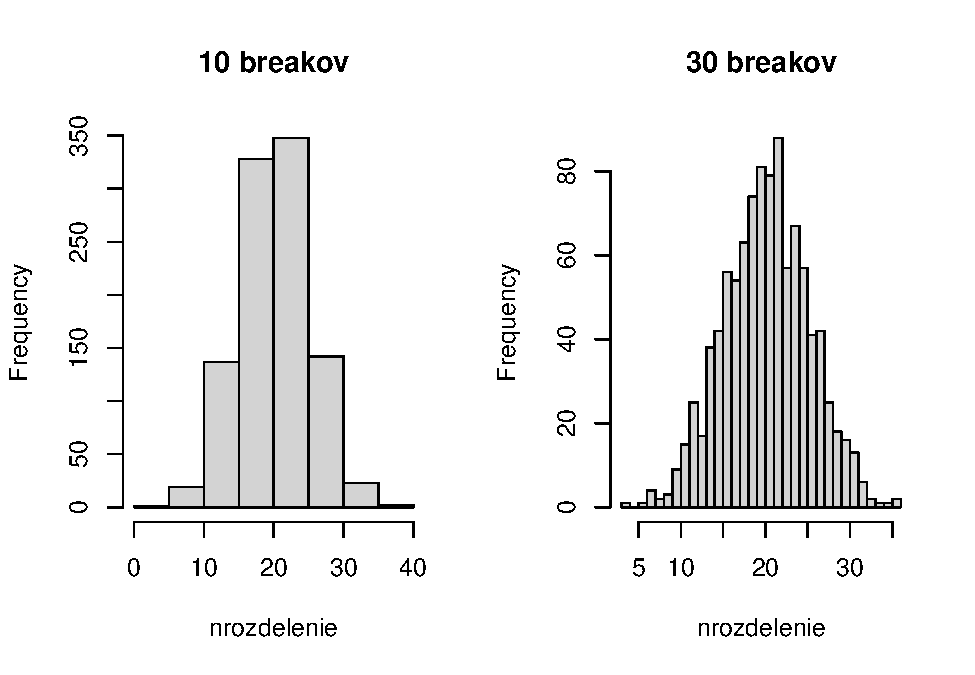
\includegraphics[width=0.8\textwidth,height=\textheight]{test_files/figure-latex/unnamed-chunk-44-1.pdf}
\caption{Normálne rozdelenia s rôznou veľkosťou/počtom košov.}
\source{Zdroj: Vlastná tvorba.}
\end{center}
\end{figure}

\begin{Shaded}
\begin{Highlighting}
\CommentTok{# Pre navrátenie zobrazenia grafov na jeden, použijeme "par(mfrow=c(1, 1))".}
\end{Highlighting}
\end{Shaded}

\newpage

\subsubsection{Počet košov v histograme.}

Koľko breakov však použiť? Viac košov (breakov, tried...) nám poskytne detailnejší pohľad na dáta, pri vysokom počte košov nás to však stojí efektívnosť sumarizácie dát. Na druhej strane, nízky počet košov poskytne histogram natoľko tesný, že nám nemusí poskytnúť žiadnu užitočnú informáciu. Aby boli koše porovnateľné, je žiadúce, aby boli koše rovnako veľké. Dôležitou informáciou pri zostavovaní histogramu predstavuje šírka košov (šírka intervalu, šírka triedy). V ideálnych prípadoch použijeme počet košov rovnaký, ako počet tried. Teda, ak máme 5 veľkostí jabĺk, každá veľkosť bude mať vlastný kôš. Nie vždy však pracujeme s takýmito ružovými dátami. Šírku koša by sme mohli vyrátať ako:
\begin{equation}
    h = \frac{rozsah \ dát}{počet \ tried} \ (Wand, 1997),
\end{equation}
kde $h$ je šírka koša a počet tried je počet požadovaných tried. Vzorec môžeme upraviť, aby sme počet tried určili podľa šírky.

Koľko teda tried? Stretávame sa s množstvom odporúčaní. Množstvo príručiek odporúča ako všeobecné pravidlo ideálne 10 intervalov, avšak v prípade potreby viac, nie ale viac ako 30. Ostatní odporúčajú rozmedzie medzi 10 až 20, ďalší 10 až 14, ostatní 5 až 15. Možno už viete, kam tým smerujem. Napriek odporúčaniam štatistici-štatisti prišli so vzorcami na určenie vhodného množstva tried, ktoré budeme označovať písmenom $k$.

"Zlatým štandardom" je Sturgeho pravidlo, ktorého vzorec je:
\begin{equation}
    k = 1 + [3.3 \times log_{10}(n)],
\end{equation}
kde $n$ je počet pozorovaní.

Ak by ste si pozreli citovaný dokument, videli by ste vyše dvoch desiatok vzorcov pre výpočet počtu košov. Tento vzorec prischol, lebo pri menších vzorkách (do 200) poskytoval podobné výsledky naprieč vzorcami. Pri veľkých vzorkách však nefunguje tak dobre. Taktiež mu veľmi nesvedčia zošikmené dáta, ktoré nemajú normálne rozdelenie. Vtedy je vhodné siahnuť po alternatívach. Jednou z takýchto alternatív je pravidlo Freedmana a Dianocisa:
\begin{equation}
    k = \left\lfloor \frac{rozsah \ dát}{2 \times (IQR) \times n^{-1/3}} \right \rfloor,
\end{equation}

kde $IRQ$ predstavuje interquartile range, čiže medzikvartilový rozsah $(Q_{3} - Q_{1})$, a neúplné hranaté zátvorky predstavujú podlahu, čo znamená, že zaokrúhľujeme na najbližšie celé číslo nadol. Ak by chýbala spodná časť, mali by sme strop, a teda zaokrúhľovali na najbližšie celé číslo nahor.
Niekto iný by však mohol tvrdiť, že používanejší je niektorý z iných vzorcov.
Keďže neexistuje jeden vzorec, na ktorom sa všetci zhodli, nie je nesprávne, a neobvyklé, používať svojvoľný počet košov. Berte to teda skôr ako ukážku, že niečo také existuje, a v prípade potreby budete vedieť, že môžete siahnuť po tabuľkách či vzorcoch, a vyskúšať podľa nich rôzne veľkosti košov [11]. 

\hypertarget{oux10dakuxe1vanuxe1-hodnota}{%
\subsection{Očakávaná hodnota}\label{oux10dakuxe1vanuxe1-hodnota}}

Spomínam si, ako som otvoril videa Bena Lamberta, a tam na mňa vyskočilo
hneď nejaké tlačené É-čko a rôzne kvačky. Veľké tlačené E znamená
expected value, teda očakávaná hodnota. Je to tak, ako to znie.
Očakávaná hodnota náhodnej premennej je jednoducho povedané priemer,
ktorý by sme vyrátali za dlhú dobu a pri niekoľkonásobnom opakovanom
výbere vzorky. Pre diskrétnu náhodnú premennú vyrátame túto hodnotu ako
vážený súčet, kde váha je určená pravdepodobnosťou výskytu. Vzorcom:
\[E(y)= y_1p_1 + y_2p_2 + ... + y_kp_k = \sum_{i=1}^{k}y_ip_i\]

A teraz príklad zo života na pochopenie. Prečo myslíte, sa hovorí
``Lucky Seven'', teda že sedmička je šťastné číslo? Je to preto, lebo
keď sčítate všetky kombinácie čísel na dvoch hracích kockách, najviac
hodnôt vyjde pre 7, teda aj pravdepodobnosť, že padne toto číslo je
väčšia, ako pri ostatných súčtoch. V priemere potom padne najviac ľudom
sedmička, ľudia si to všímajú a stavujú na sedmičky, alebo také niečo,
nie som moc na gambling.

\begin{figure}
\begin{center}

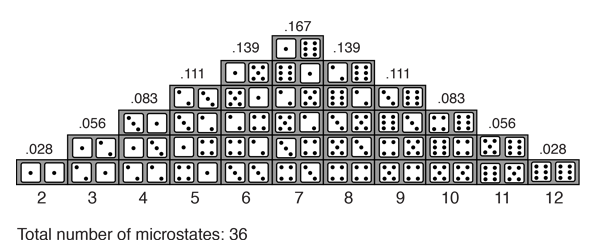
\includegraphics[width=0.8\textwidth,height=\textheight]{diplomka obrazky/5.png}
\caption{Pravdepodobnosť výskytu jednotlivých súčtov hodov.}
\source{Zdroj: Prevzaté z [12].}
\end{center}
\end{figure}

\hypertarget{zuxe1kon-veux13ekuxfdch-ux10duxedsel}{%
\subsection{Zákon veľkých
čísel}\label{zuxe1kon-veux13ekuxfdch-ux10duxedsel}}

S tým úzko súvisí aj zákon veľkých čísel. Zákon vraví, že ak rovnaký
experiment opakujeme nezávisle od seba nespočetne veľa krát, priemer
výsledkov bude blízko k \textbf{očakávanej hodnote}. Výsledok sa bude
približovať k očakávanej hodnote, ako sa bude počet pokusov zvyšovať.

\emph{Príklad:} Keď si s niekym budete hádzať mincu, možno padne 10-krát
za sebou orol, ale keby sme mincu hodili miliónkrát, výsledky by boli
približne 50/50. Inak povedané, šanca že padne hlava (alebo orol) je
50\%, ak minca nie je cinknutá. Očakávaná hodnota pri hode mincou je
0.5. Šanca že padne hlava je 1 a možné výsledky sú 2, teda
pravedpodobnosť, že padne hlava je 0.5, čiže 50\%.

\hypertarget{nuxe1hodnuxfd-vuxfdber}{%
\subsection{Náhodný výber}\label{nuxe1hodnuxfd-vuxfdber}}

V angličtine random sampling. To ing značí nejakú činnosť. Náhodný výber
znie skôr ako jeden výber, avšak pri random sampling ide o niečo iné.
Väčšina ekonometrických procedúr pracuje s priemermi vzoriek. Čiže tento
náhodný výber, sa bude týkať priemeru. Povedzme, že chceme odhadnúť
priemernú výšku v populácií. Väčšinou predpokladáme, že pozorovania sú
zozbierané náhodne z veľkej, nepoznanej populácie. Vyrátanie priemeru z
takejto vzorky má za následok to, že tento priemer je \emph{náhodnou
premennou}. \emph{Táto náhodná premenná má potom rozdelenie
pravdepodobnosti, nazývané výberové rozdelenie.} Výberové rozdelenie
závisí od rozdelenia populácie, z ktorej sme vzorku zobrali.
Predpokladajme, že máme normálne distribuovanú populáciu, a vyberieme z
nej veľa veľa vzoriek, vyrátame priemer týchto vzoriek, a urobíme z
týchto priemerov histogram. Rozdelenie tohto histogramu bude kopírovať
rozdelenie, z ktorého sme tieto vzorky zobrali, teda normálne
rozdelenie. Náhodný výber by mal eliminovať odchýlku, keďže každý z
populácie má rovnakú šancu byť vybraný. Získame teda rozdelenie bez
odchýlky, ktoré kopíruje rozdelenie populácie. Hlavným trikom tohto
náhodného výberu je, že jeho rozdelenie môže byť blízko normálneho
rozdelenia, aj keď populácia z ktorej sme brali vzorky nemá normálne
rozdelenie. A to vďaka Centrálnej limitnej vete.

\hypertarget{centruxe1lna-limitnuxe1-veta}{%
\subsection{Centrálna limitná veta}\label{centruxe1lna-limitnuxe1-veta}}

Kdežto Zákon veľkých čísel sa zameriaval skôr na odhad danej štatistiky,
Centrálna limitná veta súvisí s rozdelením vzorky. Podstatou je, že ak
vezmeme dostatočne veľké množstvo priemerov vzoriek, súbor týchto
priemerov bude mať normálne rozdelenie, bez ohľadu na rozdelenie
populácie. Takáto vzorka by mala mať aspoň 30 pozorovaní. Nie je však
potrebné zbierať veľa veľa vzoriek, keďže na vzorku použijeme estimátor,
napríklad na odhad priemeru, a samotný výsledok bude náhodná veličina
(ako sme už spomenuli pri náhodnom výbere), ktorá sama pochádza z
náhodného výberu. Čiže na splnenie predpokladu, že výsledné rozdelenie
budeme môcť odhadnúť normálnym rozdelením, závisí už len od veľkosti
vzorky. Čím vzdialenejšie od normálneho rozdelenia je rozdelenie
populácie, tým väčšia vzorka bude potrebná, aby toto pravidlo platilo.

\newpage

\hypertarget{podmienky-lineuxe1rnej-regresie}{%
\section{Podmienky lineárnej
regresie}\label{podmienky-lineuxe1rnej-regresie}}

Prečo som Vám toto všetko vravel? Pracujeme s náhodnými veličinami,
takže pochopiť zmysel náhodného výberu, je dôležité. Všetky estimátory s
ktorými pracujeme, teda \(\hat\beta{}_i\), sú náhodnými veličinami (lebo
sú vyrátané z náhodnej vzorky), teda na ich vyrátané koeficienty budú
platiť vyššie spomínané koncepty. Keď budeme pracovať s predpokladom, že
majú normálne rozdelenie, môžeme na nich aplikovať t-testy a konfidenčné
intervaly a ďalšie krásne štatistické techniky. Tento predpoklad môžeme
použiť vďaka očakávanej hodnote, keďže:
\[E(\overline{x}) = \mu\] Teda očakávaná hodnota nášho estimátora (v
tomto prípade je priemer vzorky estimátor priemeru populácie) bude rovná
priemeru populácie mí. Ono, sú to také štatistické kecy, ktoré majú
svoje opodstatnenie, avšak potrebujete troška času, aby ste sa s nimi
vžili a pochopili ich. Týmto vzorcom chceme povedať, že predpokladáme,
že rozdelenie priemeru v našej vzorke nebude odchýlené od priemeru
populácie, lebo pri očakávanej hodnote by sme vzali nekonečno veľa
vzoriek, a platil by Zákon veľkých čísel a Centrálna limitná veta. A
naša vzorka je náhodne vybraná, tak predpokladáme, že má normálne
rozdelenie a môžeme s ňou podľa toho pracovať, a aplikovať na ňu
štatistické techniky.

\hypertarget{blue}{%
\subsection{BLUE}\label{blue}}

My chceme, aby naše estimátory boli BLUE! A tým nemyslíme modré, ale
Best Linear Unbiased Estimators! Najlepší Lineárni Nevychýlení
Odhadcovia! Unbiased znamená, že v priemere Beta trafí cieľ, teda
priemer populácie. A naše \(\beta_i\) estimátory spĺňajú tieto
požadované vlastnosti, ak sú splnené isté podmienky. Určite ste počuli o
Gauss-Markov podmienkach, po ktorých splnení sú OLS estimátory BLUE.
Niekto ich uvádza 5, niekto 10. Nebudeme si ich tu všetky preberať, lebo
nuda. Spomenieme si len pár. Všetky tieto štatistické veci som Vám
vysvetľoval preto, lebo jednou z podmienok je, že:

\begin{center}

\begin{quote}
\emph{Vzorka s ktorou model pracuje musí byť zozbieraná náhodne z
populácie.}
\end{quote}

\end{center}

To znamená, že vzorka by mala byť \(i.i.d\). Independently and
Identically Distributed. Nezávislo a identicky distribovaná. To znamená,
že výber jedného pozorovania zo vzorky, neovplyvňuje výber ďalšieho
pozorovania, a že každé pozorovanie má rovnakú šancu byť vybrané. Ak to
tak bude, naše estimátory budú nevychýlené. \emph{Kvôli konceptom, ktoré
sme si predstavili vyššie.}

\begin{Shaded}
\begin{Highlighting}[]
\CommentTok{# Ukážme si, čo to biased vlastné znamená. Použijeme na to dnorm().}
\CommentTok{# dnorm() nám vyberie konkrétny bod z rozdelenia, preto je potrebné}
\CommentTok{# mu zadať vektor.}

\NormalTok{x <-}\StringTok{ }\KeywordTok{seq}\NormalTok{(}\DataTypeTok{from =} \DecValTok{-3}\NormalTok{, }\DataTypeTok{to =} \DecValTok{5}\NormalTok{, }\DataTypeTok{by =} \FloatTok{0.2}\NormalTok{)}

\CommentTok{# type = "l" ako "line", čiara.}
\CommentTok{# Povedzme, že populačný priemer mí, je 1.}
\CommentTok{# Zaznačíme si ho v grafe pomocou abline(),}
\CommentTok{# použijeme arugment "v" ako vertical.}

\KeywordTok{plot}\NormalTok{(}\DataTypeTok{x =}\NormalTok{ x, }\DataTypeTok{y =} \KeywordTok{dnorm}\NormalTok{(x, }\DataTypeTok{mean =} \DecValTok{2}\NormalTok{, }\DataTypeTok{sd =} \DecValTok{1}\NormalTok{), }\DataTypeTok{type =} \StringTok{"l"}\NormalTok{,}
     \DataTypeTok{main =} \StringTok{"biased rozdelenie"}\NormalTok{, }\DataTypeTok{ylab =} \StringTok{""}\NormalTok{, }\DataTypeTok{xlab =} \StringTok{""}\NormalTok{)}

\KeywordTok{abline}\NormalTok{(}\DataTypeTok{v =} \DecValTok{1}\NormalTok{)}
\end{Highlighting}
\end{Shaded}

\begin{figure}[!ht]
\begin{center}
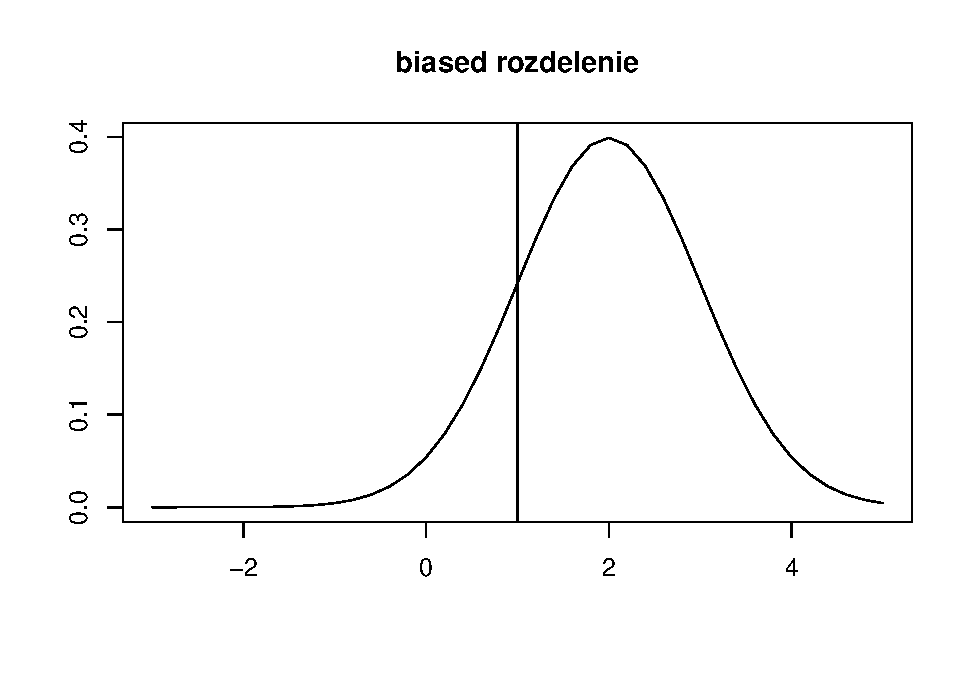
\includegraphics[width=0.9\textwidth,height=\textheight]{test_files/figure-latex/unnamed-chunk-45-1.pdf}
\caption{Vychýlené rozdelenie.}
\source{Zdroj: Vlastná tvorba.}
\end{center}
\end{figure}

Vrchol rozdelenia nie je centrovaný nad pravým priemerom, rozdelenie je
teda biased, odchýlené.

\textbf{Odchýlka však nie je jediná vec, ktorá by nás mala zaujímať.}
Potrebujeme taktiež overiť, či sú naše odhadnuté koeficienty
interpretovateľné a aplikovateľné na populáciu. K tomu nám dopomáha
štandardná chyba odhadnutých \(\hat\beta{}_i\)iet. Táto chyba je však
skreslená pri porušení ďalších Gauss-Markov podmienok. Tieto podmienky
sa týkajú chýb modelu (residuals \(\hat u_i\)). Prv sa však oboznámme s
tým, ako sú nám štandardné chyby nápomocné.

\newpage

\hypertarget{vuxfdstup-regresie}{%
\section{Výstup regresie}\label{vuxfdstup-regresie}}

Pozrime sa na výstup našej regresie a analyzujme si ho troška.

\begin{Shaded}
\begin{Highlighting}[]
\CommentTok{# Na výpis všetkých vlastností modelu použijeme summary().}
\KeywordTok{summary}\NormalTok{(model)}
\end{Highlighting}
\end{Shaded}

\begin{verbatim}
## 
## Call:
## lm(formula = data$mpg ~ data$hp)
## 
## Residuals:
##     Min      1Q  Median      3Q     Max 
## -5.7121 -2.1122 -0.8854  1.5819  8.2360 
## 
## Coefficients:
##             Estimate Std. Error t value Pr(>|t|)    
## (Intercept) 30.09886    1.63392  18.421  < 2e-16 ***
## data$hp     -0.06823    0.01012  -6.742 1.79e-07 ***
## ---
## Signif. codes:  0 '***' 0.001 '**' 0.01 '*' 0.05 '.' 0.1 ' ' 1
## 
## Residual standard error: 3.863 on 30 degrees of freedom
## Multiple R-squared:  0.6024, Adjusted R-squared:  0.5892 
## F-statistic: 45.46 on 1 and 30 DF,  p-value: 1.788e-07
\end{verbatim}

\begin{Shaded}
\begin{Highlighting}[]
\CommentTok{# Vidíme tam nejaké vlastnosti reziduí, odhadnuté koeficienty, a}
\CommentTok{# v tretej časti taktiež podstatné veci ako R^2, či F-test.}
\CommentTok{# Teraz nás však zaujíma časť s koeficientmi.}

\KeywordTok{summary}\NormalTok{(model)}\OperatorTok{$}\NormalTok{coefficients}
\end{Highlighting}
\end{Shaded}

\begin{verbatim}
##                Estimate Std. Error   t value     Pr(>|t|)
## (Intercept) 30.09886054  1.6339210 18.421246 6.642736e-18
## data$hp     -0.06822828  0.0101193 -6.742389 1.787835e-07
\end{verbatim}

\hypertarget{t-test}{%
\subsection{t-test}\label{t-test}}

Na to, aby sme určili, či sú koeficienty významné, používame t-test. To,
čo vidíme v koeficientoch v stĺpci \(t\) je označované ako
\(t-štatistika\), lebo je to štatistickou technikou vyrátaná hodnota,
ktorá je interpretovateľná. Aaale prečo vlastne t-štatistika? Pozrime sa
na t-rozdelenie.

\begin{figure}
\begin{center}

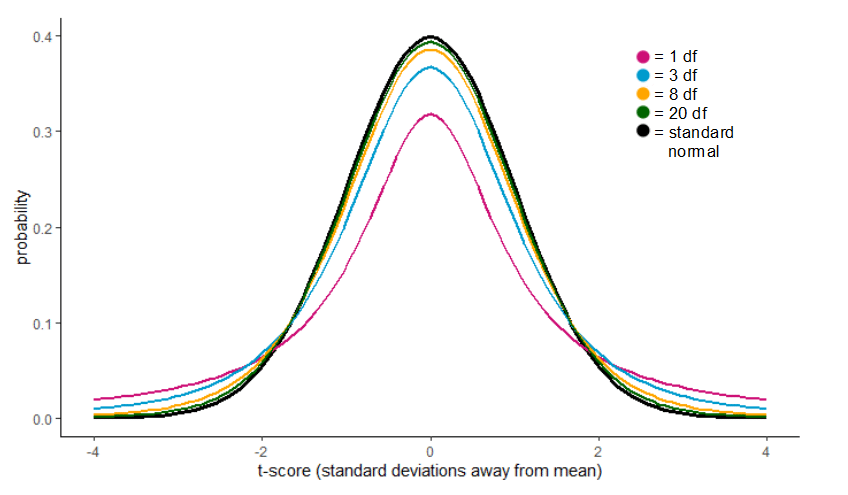
\includegraphics{diplomka obrazky/7.png}
\caption{Efektívnosť rozdelenia.}
\source{Zdroj: Prevzaté z [14].}
\end{center}
\end{figure}

Pripomína Vám to niečo? Toto t-rozdelenie je typom normálneho
rozdelenia, ktoré sa používa pri menších vzorkách. Používa sa, keď
predpokladáme, že majú dáta približne normálne rozdelenie (majú
približne bell shape, tvar zvona), avšak nepoznáme rozptyl populácie.
Odhad rozptylu t-rozdelenia záleží od veľkosti vzorky, respektíve na
stupni voľnosti. Z grafu vidíte, že ako df rastú (degree-of-freedom,
stupeň voľnosti), chvosty rozdelenia sa stenšujú a rozdelenie sa zužuje.
Stupne voľnosti vyrátame ako počet pozorovaní mínus počet premenných a
intercept. Toto rozdelenie ukazuje hustotu pravedpodobnosti, s akou sa
dané hodnoty v rozdelení môžu objaviť.

Čarovnou vlastnosťou tohto rozdelenia je, že ako rastie stupeň voľnosti,
rozdelenie sa približuje štandardnému normálnemu rozdeleniu. Štandardné
normálne rozdelenie sa vyznačuje tým, že má priemer 0 a smerodajnú
odchýlku 1.

Poďme teraz k tým juicy veciam, prečo Vám to vlastne ukazujem.

\hypertarget{t-ux161tatistika}{%
\subsection{t-štatistika}\label{t-ux161tatistika}}

Na overenie, či sme koeficient neodhadli len náhodou, ale je naozaj
významný, vyrátame t-štatistiku, ktorej formula vyzerá takto:
\[t = \frac{\hat\beta{}_i}{se(\hat\beta{}_i)}\] V t-štatistike odčítate
v čitateli vašu požadovanú hypotézu. My testujeme významnosť
\(\hat\beta{}_i\), teda či sa naša \(\hat\beta{}_i\) rovná nule a tým
pádom nie je významná. Mohli by sme to zapísať ako:
\[t = \frac{\hat\beta{}_i - \hat\beta{}_i,_0}{se(\hat\beta{}_i)}\]
Odčítame nulu, čiže sa nič nemení, a prvý zápis je úplne v poriadku.

Hej hej hej, čo je ale to se??? \emph{SE stands for standard error.}
Takže \(štandardná \ chyba\). Hmmmm, to neznie ako smerodajná odchýlka. A
máte pravdu! Lebo to nie je smerodajná odchýlka! Alebo, no, ono to
vlastne JE smerodajná odchýlka!

\hypertarget{sd-vs-se}{%
\subsection{SD vs SE}\label{sd-vs-se}}

Smerodajná odchýlka (standard deviaton) a štandardná chyba (standard
error).

Spomínate si na vzorec na rozptyl? Ak nie, tu ho máme:
\[s^{2} = \frac{\sum_{i=1}^{n} \left(x_{i} - \bar{x}\right)^{2}} {n-1}.\]

Všimnime si, že používame \(s^{2}\), namiesto \(\sigma^{2}\) (sigma
squared, squared = na druhú), lebo sa jedná o estimátor, kde odhadujeme
danú štatistiku (v tomto prípade rozptyl) zo vzorky. \(\sigma^{2}\) sa
používa na označenie rozptylu populácie. To máme to isté ako \(\mu\)
(mí), pre priemer populácie a \(\overline{x}\) pre priemer vzorky.

Smerodajná odchýlka je odmocnina vzorca uvedeného vyššie, základy
štatistiky, že?
\[s = \sqrt{\frac{\sum_{i=1}^{n} \left(x_{i} - \bar{x}\right)^{2}} {n-1}}.\]

Výberová smerodajná odchýlka (čiže smerodajná odchýlka vyrátaná zo
vzorky, nenechajte sa zmiesť, je to to isté ako vyššie, len sme pridali
výberová, nech sme korektní) nám určuje osciláciu hodnôt okolo priemeru,
ako veľmi sú okolo toho priemeru rozptýlené.

Štandardná chyba opisuje to isté, avšak miesto vzorky, pracuje so vzorkou
plnou priemerov. Spomeňme si na výberové rozdelenie pri náhodnom výbere.
Vezmeme vzorku, vyrátame z nej priemer a priemer dáme do šuflíka.
Vezmeme ďalšiu vzorku, vyrátame jej priemer, a aj tento priemer hodíme
do šuflíka. Toto zopakujeme veľakrát, a máme plný šuflík priemerov. Z
tejto šuplíkovej vzorky priemerov vyrátame priemer. Aaa potom vyrátame,
ako zvyšné hodnoty (priemery), oscilujú okolo priemeru vzorky. Vyrátali
sme teda smero\ldots ehm.. štandardnú chybu! Keď sa bavíme o štandardnej
chybe (SE), vieme, že sa bavíme o tom, ako natesno je súbor priemerov,
okolo priemeru. Čiže je to smerodajná odchýlka pre priemery.

\begin{quote}
\emph{V štatistike sa to beri ako odhad smerodajnej odchýlky priemeru
vzorky, okolo skutočného priemeru populácie.}
\end{quote}

Na hodine to budete rátať pomocou variačno-kovariačnej matice. My si
ukážeme všeobecný vzorec:
\[s_{\bar{X}} = \frac{s}{\sqrt{n}}\]

\begin{quote}
\emph{Vydelíme smerodajnú odchýlku vzorky, odmocninou počtu pozorovaní
vo vzorke.}
\end{quote}

Alternatívny zápis:
\[SE = \frac{s}{\sqrt{n}}\] Takže vráťme sa k našej \(t-štatistike\):
\[t = \frac{\hat\beta{}_i}{se(\hat\beta{}_i)}\]

Na jej vyrátanie použijeme odhadnutý \(\hat\beta{}_i\) koeficient, a
predelíme ho odhadnutou štandardnou chybou (ktorú pre nás vyráta R-ko do
koeficientov). Pozrime sa ešte raz na koeficienty:

\begin{Shaded}
\begin{Highlighting}[]
\KeywordTok{summary}\NormalTok{(model)}\OperatorTok{$}\NormalTok{coefficients}
\end{Highlighting}
\end{Shaded}

\begin{verbatim}
##                Estimate Std. Error   t value     Pr(>|t|)
## (Intercept) 30.09886054  1.6339210 18.421246 6.642736e-18
## data$hp     -0.06822828  0.0101193 -6.742389 1.787835e-07
\end{verbatim}

\begin{Shaded}
\begin{Highlighting}[]
\CommentTok{# Vydeľme koeficient "estimate", číslom "Std. Error" (SE),}
\CommentTok{# a pozrime sa, či nám výjde t-štatistika.}
\NormalTok{nase_t <-}\StringTok{ }\KeywordTok{summary}\NormalTok{(model)}\OperatorTok{$}\NormalTok{coefficients[}\DecValTok{1}\NormalTok{, }\DecValTok{1}\NormalTok{] }\OperatorTok{/}\StringTok{ }
          \KeywordTok{summary}\NormalTok{(model)}\OperatorTok{$}\NormalTok{coefficients[}\DecValTok{1}\NormalTok{, }\DecValTok{2}\NormalTok{]}
\NormalTok{nase_t}
\end{Highlighting}
\end{Shaded}

\begin{verbatim}
## [1] 18.42125
\end{verbatim}

\hypertarget{kritickuxe1-hodnota}{%
\subsection{Kritická hodnota}\label{kritickuxe1-hodnota}}

Kritická hodnota pre t-štatistiku je približne 2, že? Čo to ale značí?
Keď koeficient predelíme štandardnou chybou, rátame, koľko štandardných
chýb sa vmestí do tejto hodnoty, čiže koľko štandardných chýb je
vzdialená od tejto hodnoty. T-rozdelenie je rozdelenie pravedpobodnosti,
a čím je bližšie k stredu, tým je väčšia pravdepodobnosť výskytu. Ak si
spomínate, čo sme si vraveli pri normálnom rozdelení, že 68\% sa
nachádza v rozmedzí jednej smerodajnej odchýlky, a 95\% v rozmedzí dvoch
smerodajných odchýlok. 95\% a 2 štandardné chyby, hm, hm? Aká je
väčšinou naša hladina významnosti? 5\%! Čo je 100 - 95. A znova
opakujem, bavíme sa o rozdelení pravdepodobnosti. Ak je teda
t-štatistika väčšia ako 2, nachádzame sa ďalej ako 2 smerodajné odchýlky
od centra rozdelenia, a \textbf{pravedpodobnosť} výskytu tejto hodnoty,
je menšia ako 5\%. Šanca, že sme tento koeficient odhadli len čistou
náhodou (menej ako 5\% sa berie ako náhoda, ``by chance''), je menej ako
5\%. A teda považujeme tento koeficient za štatisticky významný.

\begin{figure}
\begin{center}

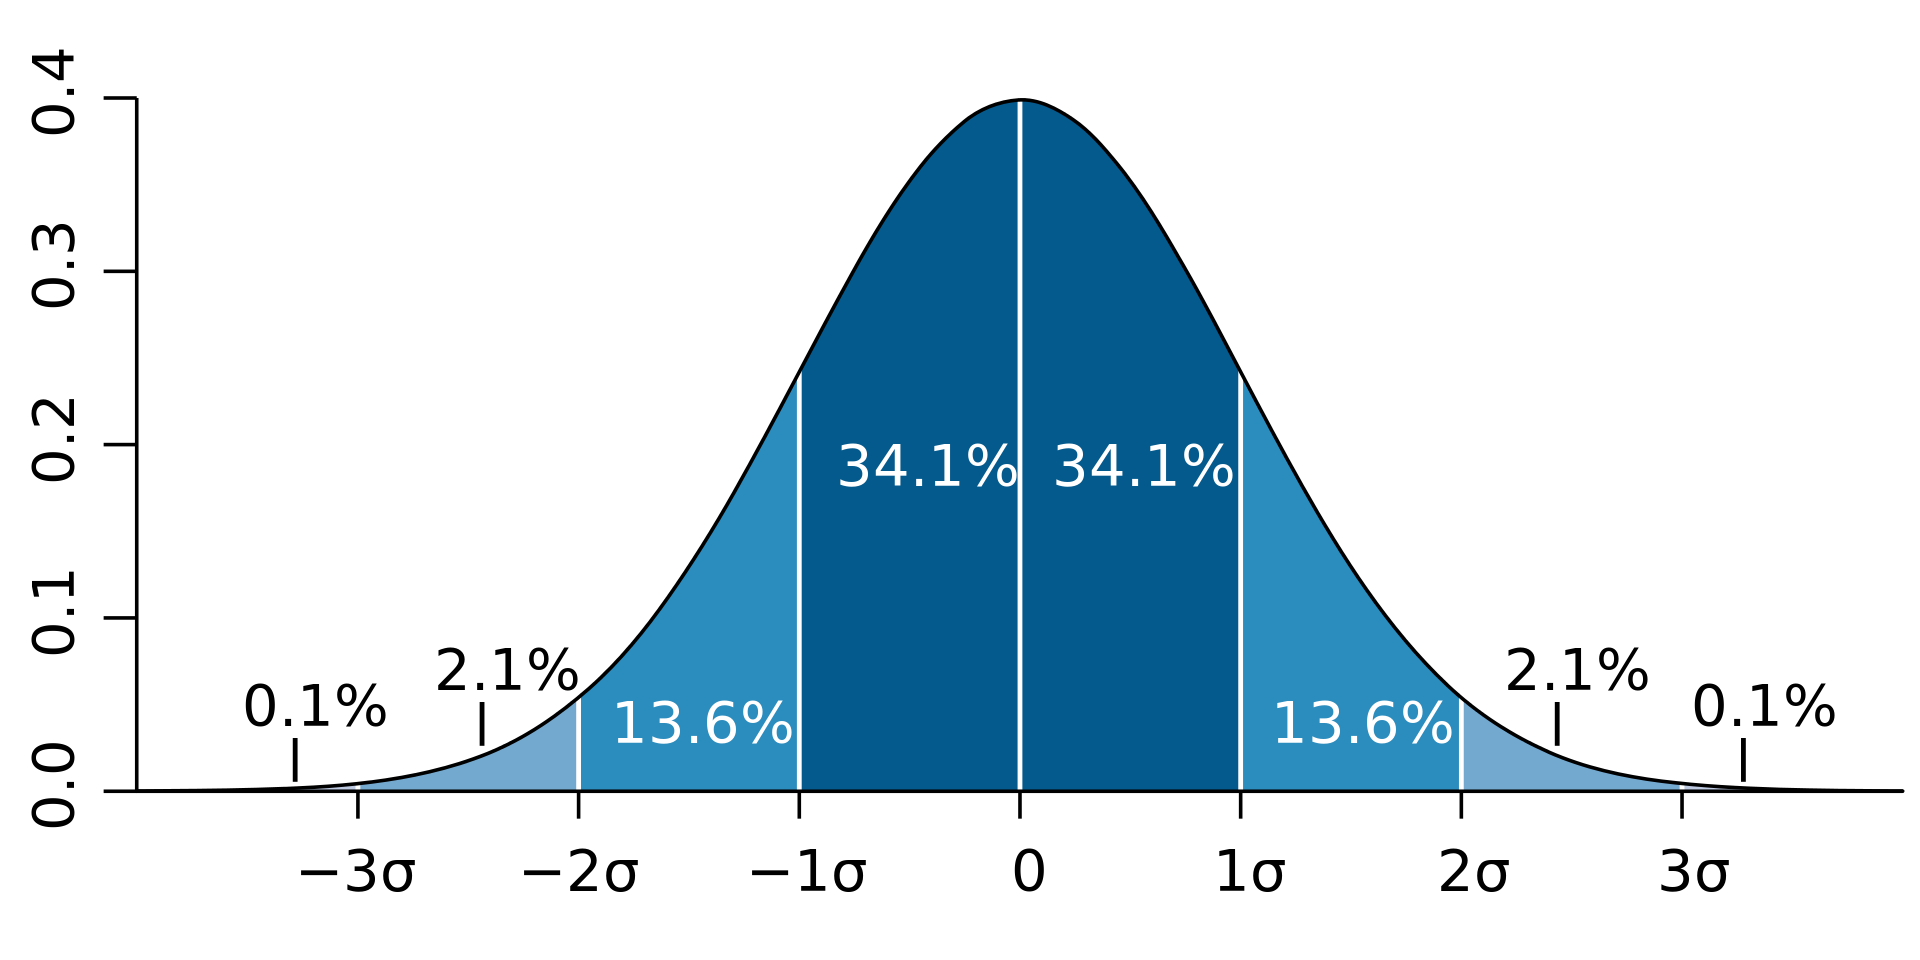
\includegraphics[width=0.8\textwidth,height=\textheight]{diplomka obrazky/8.png}
\caption{Smerodajné odchýlky a frekvencia rozdelenia.}
\source{Zdroj: Prevzaté z [13].}
\end{center}
\end{figure}

\newpage

\hypertarget{p-hodnota}{%
\subsection{p-hodnota}\label{p-hodnota}}

Pomocou t-štatistiky môžeme vyrátať p-hodnotu. Naša nulová hypotéza
bola:

\[H_0: \hat\beta{}_i = 0\]

Nulovú hypotézu zamietame, ak je t-štatistika väčšia ako 2, čiže sa
nachádza v chvostoch rozdelenia, inými slovami, je malá pravdepodobnosť,
že sme túto hodnotu vyrátali náhodne. A p-hodnota nevraví nič iné, ako
to, aká je pravdepodobnosť, že by sme dostali našu \(\hat\beta{}_i\)etu,
za predpokladu, že nulová hypotéza platí. p-hodnota, ukazuje
pravedpodobnosť výskytu nulovej hypotézy. Ak je táto hodnota malá,
zamietame, že \(\hat\beta{}_i\) je štatisticky nevýznamná a rovná nule.

\begin{Shaded}
\begin{Highlighting}[]
\CommentTok{# V našom prípade boli p-hodnoty 6.642736e-18, čo je veľmi malé číslo,}
\CommentTok{# 18 núl pred šestkou. Dávajte pozor, keby tam bolo e+18, tak je to }
\CommentTok{# obrovské číslo. :D Väčšinou sú malé p-hodnoty označené 3 hviezdičkami.}

\KeywordTok{summary}\NormalTok{(model)}\OperatorTok{$}\NormalTok{coefficients}
\end{Highlighting}
\end{Shaded}

\begin{verbatim}
##                Estimate Std. Error   t value     Pr(>|t|)
## (Intercept) 30.09886054  1.6339210 18.421246 6.642736e-18
## data$hp     -0.06822828  0.0101193 -6.742389 1.787835e-07
\end{verbatim}

\hypertarget{konfidenux10dnuxfd-interval}{%
\subsection{Konfidenčný interval}\label{konfidenux10dnuxfd-interval}}

Keď už sme zabŕdli do tej štatistiky, povedzme si rýchlo, čo je
konfidenčný interval. Najprv si ukážeme zápis konfidenčného intervalu
pre jednu premennú (nevravíme pre jednu preto, lebo pracujeme s
jednoduchou lineárnou regresiou, ale preto, že sa konfidenčný interval
vytvára pre každú premennú zvlášť):
\[[\hat\beta{}_i - 1.96 × SE(\hat\beta{}_i)\;\;,\;\;\hat\beta{}_i + 1.96 × SE(\hat\beta{}_i)].\]
Od odhadnutého koeficientu prv odčítame dve štandardné chyby pre určenie
spodnej hranice, a potom pričítame dve štandardné chyby pre určenie
hornej hranice.

\begin{Shaded}
\begin{Highlighting}[]
\CommentTok{# V R-ku konfidnčný interval odhadneme pomocou confint().}
\CommentTok{# Ukážeme si neskôr aj robustnú alternatívu. Zatiaľ pracujeme}
\CommentTok{# len s basic balíkmi v R.}

\KeywordTok{confint}\NormalTok{(model)}
\end{Highlighting}
\end{Shaded}

\begin{verbatim}
##                   2.5 %     97.5 %
## (Intercept) 26.76194879 33.4357723
## data$hp     -0.08889465 -0.0475619
\end{verbatim}

Interpretácia konfidenčného intervalu je nasledovná:``Ak by sme vzali
nekonečno vzoriek z populácie, v 95\% prípadov, by sa skutočný priemer
populácie nachádzal v rozmedzí 26.8 až 33.44.''

\newpage

\hypertarget{vlastnosti-reziduuxed}{%
\section{Vlastnosti rezíduí}\label{vlastnosti-reziduuxed}}

Aby sme koeficienty modelu mohli použiť na štatistickú inferenciu, je
potrebné skontrolovať vlastnosti reziduí. Tieto vlastnosti sú ďalšími z
podmienok OLS metódy. Na cvičeniach sa budete venovať ich rátaniu a
ukážkach na modeloch. Ja Vám poviem, čo takéto nesplnenie vlastnosti
spôsobí, a pokúsim sa Vám to vryť do pamäti pomocou vizualizácie.
Stručne zhrniem aj využité testy a riešenia. Treba si
\textbf{zvýrazniť}, že tieto podmienky sa vzťahujú len na reziduá, a nie
na nezávislé premenné.

\hypertarget{normalita}{%
\subsection{Normalita}\label{normalita}}

Chceme, aby boli naše rezíduá normálne rozdelené, čo to znamená?
Nechceme vidieť žiaden vzor správania rezíduí. Rezíduá majú byť
nezávisle od nezávislých premenných a s priemerom 0. Naše rezíduá si
plotneme spolu s fitted, teda odhadnutými hodnotami na priamke. V prvom
grafe sme si pridali priamku, keďže rezíduá by mali byť porozhadzované
nezávisle po oboch stranách. Druhý graf je takzvaný QQ-plot. Rezíduá sú
rozdelené normálne, ak kopírujú diagonálnu priamku, ktorú sme si
nakreslili. Tá priamka je totižto vytvorená z normálneho rozdelenia. Ak
by sme si otestovali tieto rezíduá z nášho modelu, nezamietli by sme
nulovú hypotézu, rezíduá teda sú rozdelené normálne-ish.

\begin{Shaded}
\begin{Highlighting}[]
\CommentTok{# My sme si tieto grafy vytvorili manuálne, dopracovali by ste sa k ním}
\CommentTok{# však aj cez funkciu plot(váš_model).}
\CommentTok{# Museli by ste sa k nemu však preklikať.}

\KeywordTok{par}\NormalTok{(}\DataTypeTok{mfrow=}\KeywordTok{c}\NormalTok{(}\DecValTok{1}\NormalTok{, }\DecValTok{2}\NormalTok{))}

\KeywordTok{plot}\NormalTok{(model}\OperatorTok{$}\NormalTok{fitted.values, model}\OperatorTok{$}\NormalTok{residuals, }\DataTypeTok{main =} \StringTok{"reziduá vs fitted"}\NormalTok{)}
\KeywordTok{abline}\NormalTok{(}\DecValTok{0}\NormalTok{, }\DecValTok{0}\NormalTok{)}

\KeywordTok{qqnorm}\NormalTok{(model}\OperatorTok{$}\NormalTok{residuals)}
\KeywordTok{qqline}\NormalTok{(model}\OperatorTok{$}\NormalTok{residuals)}
\end{Highlighting}
\end{Shaded}

\begin{figure}
\begin{center}
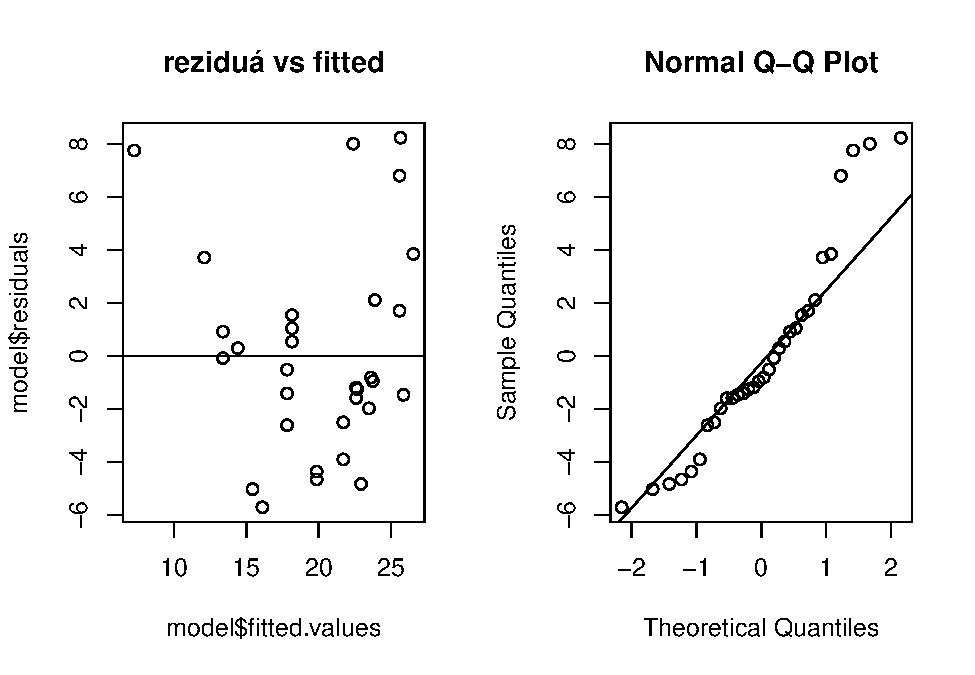
\includegraphics{test_files/figure-latex/unnamed-chunk-50-1.pdf}
\caption{Typy zobrazenia rezíduí.}
\source{Zdroj: Vlastná tvorba.}
\end{center}
\end{figure}

\newpage

Všetky podmienky, ktoré spomenieme nebudú ovplyvnovať odchýlku
koeficientu, avšak budú ovplyvňovať štandardnú chybu, teda aj
t-štatistiku a p-hodnotu. To nám znemožní správne odhadnúť štatistickú
signifikatnosť koeficientu.

Podmienka normality reziduí je jednou z tých menej závažnejších, a často
sa stane, že nie je splnená. Problémom to prestáva byť pri veľkých
vzorkách, kde začne úradovať Central limit theorem.

\hypertarget{homoskedasticita}{%
\subsection{Homoskedasticita}\label{homoskedasticita}}

Ďalšou podmienkou je konštantný rozptyl reziduí - homoskedasticita. Ak
rozptyl nie je konštantný, ale zväčšuje sa, bavíme sa o prítomnosti
heteroskedasticity. Ukážeme si to na najklasickejšom príklade, a to
vzťah príjmu a výdavkov na jedlo. Ľudia potrebujú jesť približne
rovnako, keď máte málo peňazí, nemáte veľmi na výber a všetci ľudia s
nízkym príjmom kupujú podobné množstvo a typ jedla, vynakladajú pomerne
rovnakú časť ich príjmov. Ako však príjem rastie, ľudia nezjedia
signifikantne viac, avšak môžu utrácať za omnoho drahšie potraviny, a
niekto je podobne ako ľudia s nižším príjmom. Je tam teda veľký rozptyl,
lebo ľudia s vyšším príjmom majú na výber. Pri nižšom príjme tento
rozptyl nie je, lebo keď zarobia 1000eur, nemôžu minút na potraviny 10
000eur.

\begin{Shaded}
\begin{Highlighting}[]
\CommentTok{# Vytvorme si premenné, kde X budú mzdy.}
\NormalTok{X <-}\StringTok{ }\DecValTok{1}\OperatorTok{:}\DecValTok{500}
\NormalTok{Y <-}\StringTok{ }\KeywordTok{rnorm}\NormalTok{(}\DataTypeTok{n =} \DecValTok{500}\NormalTok{, }\DataTypeTok{mean =}\NormalTok{ X, }\DataTypeTok{sd =} \FloatTok{0.6} \OperatorTok{*}\StringTok{ }\NormalTok{X)}
\NormalTok{mzdy_jedlo <-}\StringTok{ }\KeywordTok{lm}\NormalTok{(Y }\OperatorTok{~}\StringTok{ }\NormalTok{X)}

\KeywordTok{plot}\NormalTok{(}\DataTypeTok{x =}\NormalTok{ X, }\DataTypeTok{y =}\NormalTok{ Y, }\DataTypeTok{xlab =} \StringTok{"príjem"}\NormalTok{, }\DataTypeTok{ylab =} \StringTok{"výdaje na jedlo"}\NormalTok{,}
     \DataTypeTok{main =} \StringTok{"vzťah príjmu a výdavkov na jedlo"}\NormalTok{)}

\KeywordTok{abline}\NormalTok{(mzdy_jedlo, }\DataTypeTok{col =} \StringTok{"red"}\NormalTok{)}
\end{Highlighting}
\end{Shaded}

\begin{figure}
\begin{center}
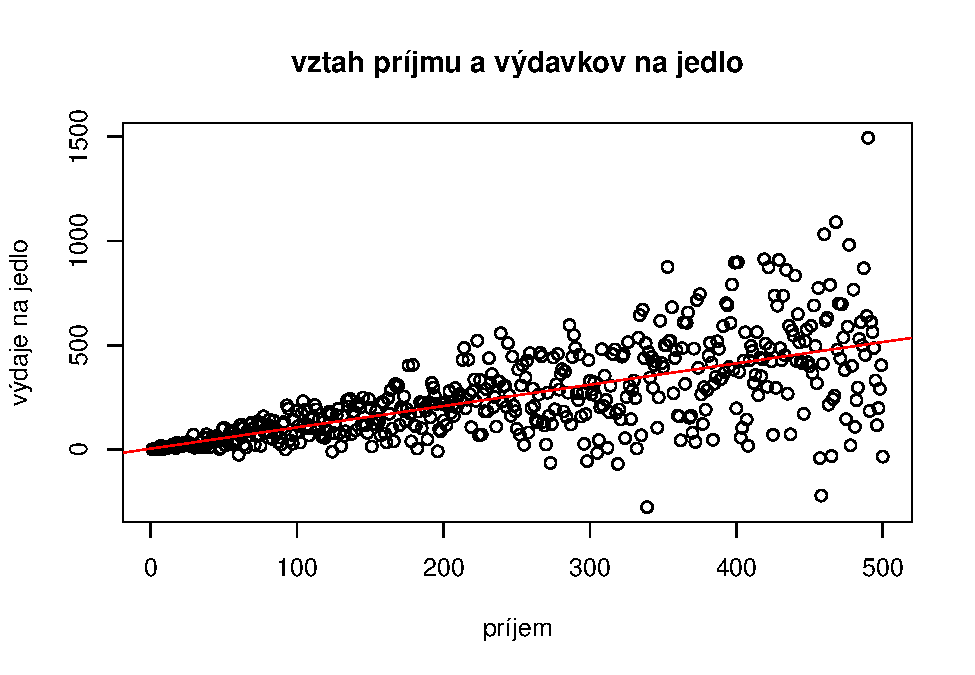
\includegraphics[width=1\textwidth,height=\textheight]{test_files/figure-latex/unnamed-chunk-51-1.pdf}
\caption{Prítomnosť heteroskedasticity.}
\source{Zdroj: Vlastná tvorba.}
\end{center}
\end{figure}

Prítomnosť heteroskedasticity \textbf{zmenší} štandardnú chybu,
dostaneme menšie hodnoty, než by sme mali. To môže viesť k označeniu
koeficientu za štatisticky signifikantný, aj keď to nebude pravda.

\newpage

Heteroskedasticitu môžeme detekovať pomocou:

\begin{itemize}
\tightlist
\item
  vizualizácie,
\item
  Breusch-Pagan testu,
\item
  Goldfeld-Quandt testu.
\end{itemize}

A vyriešiť napríklad pomocou:

\begin{itemize}
\tightlist
\item
  robustných metód na odhad štandardných chýb,
\item
  vážených najmenších štvorcov (WLS),
\item
  logaritmickej transformácie modelu.
\end{itemize}

\hypertarget{autokoreluxe1cia}{%
\subsection{Autokorelácia}\label{autokoreluxe1cia}}

Autokorelácia, alebo sériová korelácia znamená, keď vieme predpovedať
pohyb zvyšku pomocou iného zvyšku. Takže reziduá od seba nie sú
nezávislé. Takýto problém sa častejšie vyskytuje v časových radoch. Môže
to byť spôsobené Odchýlkou vynechanej premennej alebo nesprávnou
špecifikáciou modelu. Aj tento neduh je možné analyzovať buď vizuálne
alebo testami. Samozrejme testy sú omnoho spoľahlivejie. My si ale
ukážeme ako taká autokorelácia vyzerá.

\begin{figure}
\begin{center}
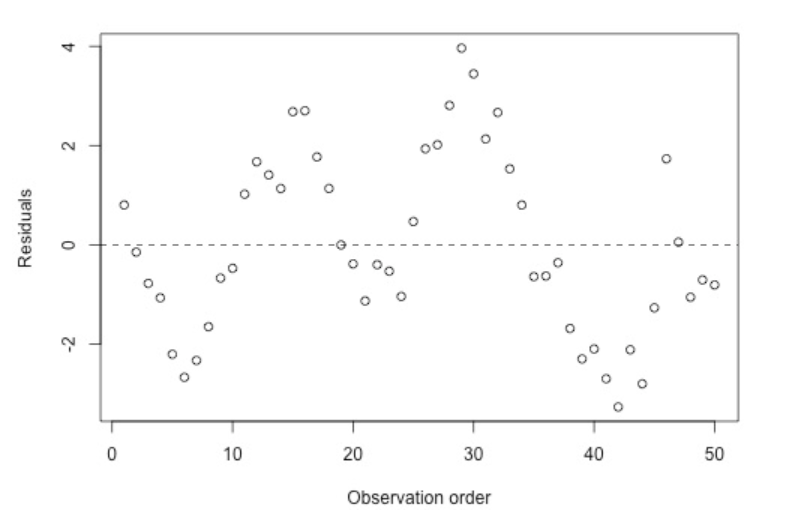
\includegraphics{diplomka obrazky/9.png}
\caption{Prítomnosť autokorelácie.}
\source{Zdroj: Prevzaté z [15].}
\end{center}
\end{figure}


\begin{Shaded}
\begin{Highlighting}[]
\CommentTok{# Šikovnou funkciou na skontrolovanie autokorelácie je acf().}
\CommentTok{# Cool trik je, ak chcete nový riadok v názvoch, použite "\textbackslash{}n".}

\KeywordTok{acf}\NormalTok{(model}\OperatorTok{$}\NormalTok{residuals, }\DataTypeTok{main =} \StringTok{"do funkcie vložíme }\CharTok{\textbackslash{}n}\StringTok{ klasicky reziduá"}\NormalTok{)}
\end{Highlighting}
\end{Shaded}

\begin{figure}
\begin{center}
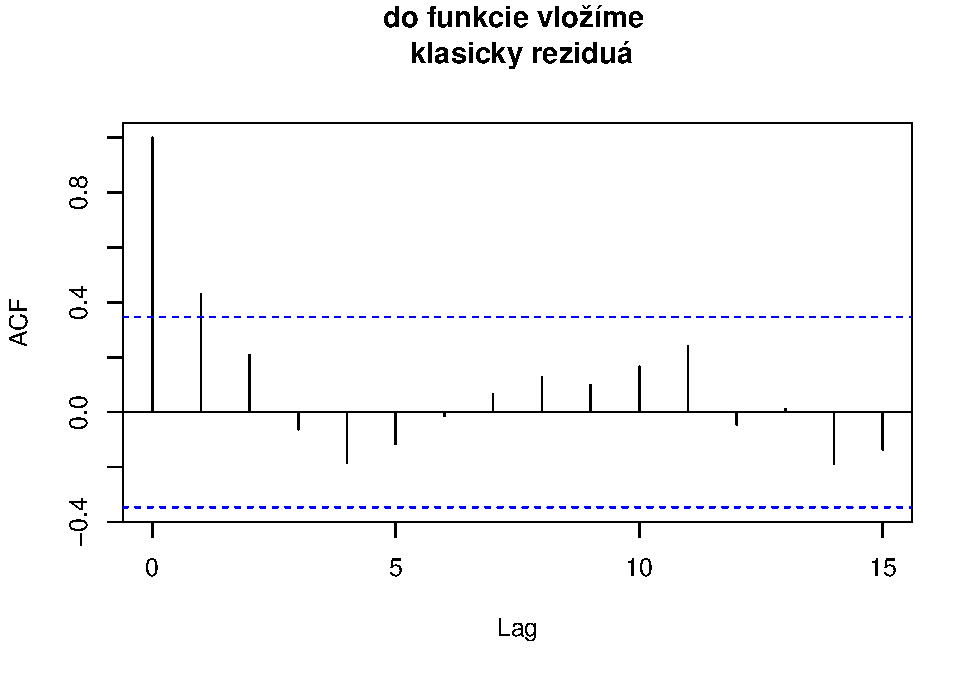
\includegraphics[width=0.8\textwidth,height=\textheight]{test_files/figure-latex/unnamed-chunk-52-1.pdf}
\caption{Výstup funkcie acf().}
\source{Zdroj: Vlastná tvorba.}
\end{center}
\end{figure}

\begin{Shaded}
\begin{Highlighting}[]
\CommentTok{# Samozrejme v prvom stĺpci bude korelácia jedna,}
\CommentTok{# lebo korelujeme samého seba.}
\CommentTok{# Ak sú korelácia nepresahuje za čiary, reziduá nie sú silne}
\CommentTok{# korelované, a autokorelácia, resp. sériová korelácia, nie je prítomná.}
\end{Highlighting}
\end{Shaded}

Problémy nám to spôsobí podobné ako heteroskedasticita, okrem iného však
môže ovplyvniť aj hodnotu \(R^2\). Autokoreláciu môžeme detekovať
pomocou:

\begin{itemize}
\tightlist
\item
  Durbin-Watson testu,
\item
  Breusch-Godfrey testu.
\end{itemize}

A vyriešiť pomocou:
\begin{itemize}
\tightlist
\item
  robustných metód na odhad štandardných chýb,
\item
  doplnenia vynechanej premennej,
\item
  opravenia funkčnej formy modelu,
\item
  využitia prvých diferencií,
\item
  použitia dummy premenných.
\end{itemize}

\hypertarget{multikolinearita}{%
\subsection{Multikolinearita}\label{multikolinearita}}

Multikolinearita sa vyskytuje len vo viacnásobnej regresií, keďže sa
jedná o koreláciu medzi dvoma nezávislými premennými. Korelácia medzi
závislou a nezávislou premennou je žiaduca. Poznáme dokonalú a
nedokonalú multikolinearitu. Pri dokonalej dokážeme jednu nezávislú
premennú vyjadriť lineárnou kombináciou inej premennej. V takomto
prípade nám väčšinou ani počítač nebude chcieť model vyrátať. Nás
väčšinou trápi nedokonalá, kde sú premenné vysoko korelované. Prečo je
to problém? AK sú premenné korelované, nedokážeme dobre odhadnúť
koeficient, keďže pri každej pridanej alebo odobranej premennej, má
koeficient tendenciu sa meniť a to vo väčšej miere. Inak povedané, je
problém dostatočne odizolovať koeficient. Koeficienty sú tak citlivé na
zmenu premenných. Ďalším problémom je, že štandardné chyby nám riadne
narastú, čím môžu označiť štatisticky signifikantné premenné za
nesignifikantné. \(R^2\) a F-test však nezvyknú byť ovplyvnené.

Multikolinearitu je možné detekovať pomocou:

\begin{itemize}
\tightlist
\item
  korelačnej matice,
\item
  VIF test,
\item
  analýzy determinantu matice,
\item
  parciálnych korelačných koeficientov.
\end{itemize}

A vyriešiť pomocou:

\begin{itemize}
\tightlist
\item
  odstránenia jednej z korelovaných premenných,
\item
  skombinovanie premenných,
\item
  neurobiť nič.
\end{itemize}

Niekedy je možné premennú ponechať v modeli, ak našim cieľom nie je
použiť ju na interpretovanie, ale len ako kontrolnú premennú, alebo keď
korelácia nie je neúnosne vysoká (0.9 a viac).




